\chapter{Apprentissage automatique pour le traitement de la parole}
\label{chapitre2}
«La tristesse de l'intelligence artificielle est qu'elle est sans artifice, donc sans intelligence.»  (Jean Baudrillard, 1987)


\section{Apprentissage automatique : définition}

Dans le domaine de l'intelligence artificielle (IA), l'apprentissage automatique (machine learning, abrégé ML en anglais) regroupe des méthodes permettant à un système d'apprendre un comportement. Selon le Journal Officiel~\footnote{https://www.legifrance.gouv.fr/jorf/id/JORFTEXT000037783813}, l'apprentissage se définit par un~\textit{processus par lequel un algorithme évalue et améliore ses performances sans l'intervention d'un programmeur, en répétant son exécution sur des jeux de données jusqu'à obtenir, de manière régulière, des résultats pertinents}. Généralement, l'apprentissage automatique permet, à partir de données plus ou moins massives, d'apprendre à caractériser de nouvelles données de même nature par une classification ou une régression. On apprend des faits à partir de données connues, pour les appliquer sur des nouvelles situations. On dit alors qu'un système automatique a été entraîné avec des données d’entraînement (première étape) afin de permettre la prédiction des caractéristiques de nouvelles données similaires (seconde étape) appelées données de développement, de test ou de validation.

\begin{figure}
  \centering
  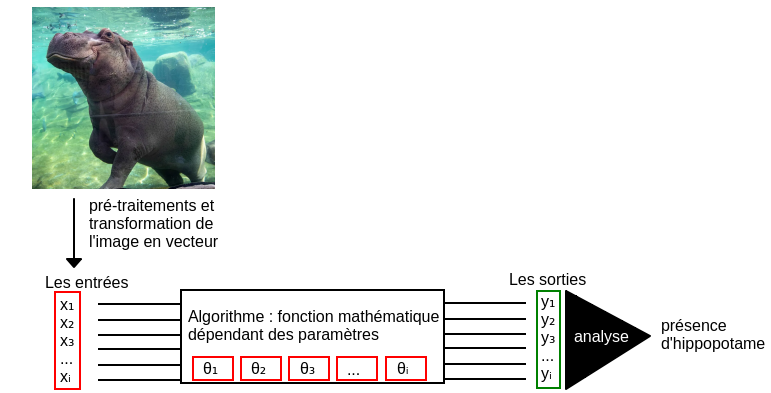
\includegraphics[width=16cm]{./Chapitre2/figures/apprentissageE_S.png}
  \caption{Représentation graphique d'un système d'apprentissage automatique avec ses entrées et ses sorties.}
  \label{fig:apprentissageE_S}
\end{figure}


%Concretement, l'apprentissage sert à apprendre les différentes variables d'une fonction mathématique permettant de séparer les données en différents ensembles grâce à une fonction de cout.
Concrètement, si on regarde la figure~\ref{fig:apprentissageE_S}, nous prenons en exemple la caractérisation de l'image d'entrée par la présence ou l'absence d'hippopotame. L'apprentissage sert à construire un modèle mathématique et apprendre les différentes variables $\theta_i$ de celui-ci à partir de données pré-traitées que l'on nomme d'entrées $x_i$. Les différents paramètres sont actualisés au fur et à mesure de l'apprentissage par minimisation de la fonction de coût. Les sorties $y_i$ de cette fonction mathématique peuvent être analysées afin de caractériser les données d'entrées.
  %Tous ces termes seront définis dans les prochaines sections.

\subsection{Classification et régression}
La classification et la régression sont les deux grandes tâches d'apprentissage automatique.
La classification correspond à résoudre un problème d'affectation de classes. Par exemple, on peut apprendre à détecter la présence d'hippopotame au sein d'une image. Nous avons alors deux réponses possibles : la présence ou l'absence de l'animal. Ces réponses se transforment donc en classes, qui seront apprises par un apprentissage automatique de type classification. Nous avons un nombre défini et connu de catégories, donc un espace discret, qui sera utilisé par le système pour catégoriser chacune des données.

La régression quant à elle ne permet pas de catégoriser les données en classes, elle les inscrit dans un espace continu. Par exemple, on peut apprendre à  prédire la valeur d'un stock en bourse à partir des valeurs des jours précédents. On peut également prédire une valeur représentant le niveau de satisfaction d'un client à partir d'un questionnaire. Les réponses sont des nombres réels qui peuvent être positifs ou négatifs. Nous avons donc une échelle de valeurs dans laquelle le système va inscrire sa prédiction.

%\begin{figure}
  \centering
  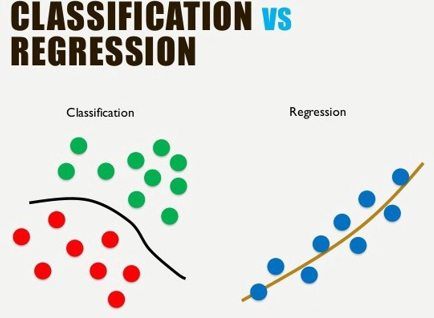
\includegraphics[width=8cm]{./Chapitre2/figures/classifVSreg.png}
  \caption{Représentation graphique de la classification et de la régression.}
  \label{fig:classifVSreg}
\end{figure}


%On peut retrouver graphiquement la différence entre la classification et la régression. Pour une classification, le système automatique va chercher à mettre en place une démarcation entre les données de classes différentes, ici pour séparer les points verts et rouges. Cela permet de positionner une nouvelle donnée dans la classe la plus proche. Tandis que pour une régression, le système va chercher la courbe qui minimise la somme des écarts de chaque point avec la courbe. On aura donc une courbe de tendance qui permet de prédire les caractéristiques des nouvelles données.


Afin d'avoir des systèmes performants, il est important de bien configurer leur apprentissage.

\subsection{Les pré-requis pour un Apprentissage Automatique réussi}
Un facteur crucial garantissant la qualité de ces systèmes automatiques réside dans les données d’entraînement. Plus elles sont qualitatives, c'est-à-dire qu'elles sont les plus proches des données réelles que nous voulons analyser, et plus le système sera performant dans sa tâche de prédiction. Mais la qualité ne fait pas tout dans ce contexte, la diversité et l'exhaustivité sont tout aussi important. Par exemple dans une tâche de reconnaissance d'hippopotame au sein d'une image, si on présente uniquement des animaux noirs alors le système pourra mal classifier des hippopotames marrons.

Mais les données ne font pas tout, le choix de l'algorithme mis en place pour apprendre le système automatique est tout aussi important. Il existe de nombreuses méthodes mathématiques permettant de modéliser un système automatique . Ces méthodes d'apprentissage automatique sont diverses et les réseaux de neurones, appelées Deep Neural Network en anglais (DNN) ou Deep Learning en font partie.
Lorsque nous cherchons à mettre en place un apprentissage automatique ces deux facteurs sont décisifs : les données et le choix de l'algorithme.

Ces choix doivent être en adéquation avec le type de caractérisation recherchée. En effet, il existe deux principales approches d'apprentissage : l'apprentissage supervisé et l'apprentissage non-supervisé.

\subsection{Apprentissage supervisé et non supervisé}

Il existe de nombreuses approches d'apprentissage dont les principaux sont présentés dans la figure~\ref{fig:typesApprentissage}. Dans le contexte de cette thèse, nous ne parlerons que d'apprentissage supervisé, non-supervisé et auto-supervisé.

Dans le cas de l'apprentissage supervisé, l'humain va \textit{guider} l’algorithme en fournissant des exemples concrets qui sont étiquetés avec les résultats attendus, comme dans la figure~\ref{fig:apprentissageE_S}. Concrètement, pour apprendre à discerner des images contenant des hippopotames, on va collecter un ensemble d'image contenant ou non un hippopotame, et pour chaque image, on va lui attribuer une étiquette \textit{présence} ou \textit{absence}. Cette étiquette peut également être appelée référence, annotation ou label. Ainsi nous avons un ensemble d'exemples concrets que nous pouvons soumettre à notre algorithme d'apprentissage.
Le système va alors apprendre à partir de chaque exemple ses paramètres de façon à diminuer l’écart entre le résultat obtenu et le résultat attendu. La marge d’erreur se réduit avec chaque itération de l'apprentissage, avec pour but d’être capable de généraliser son apprentissage à de nouveaux cas. Ce type d'apprentissage ne peut donc être mis en place que lorsque nous avons des données d’entraînement qui sont annotées. Cette annotation peut être effectuée soit par l'humain soit par la machine.

\begin{figure}
  \centering
  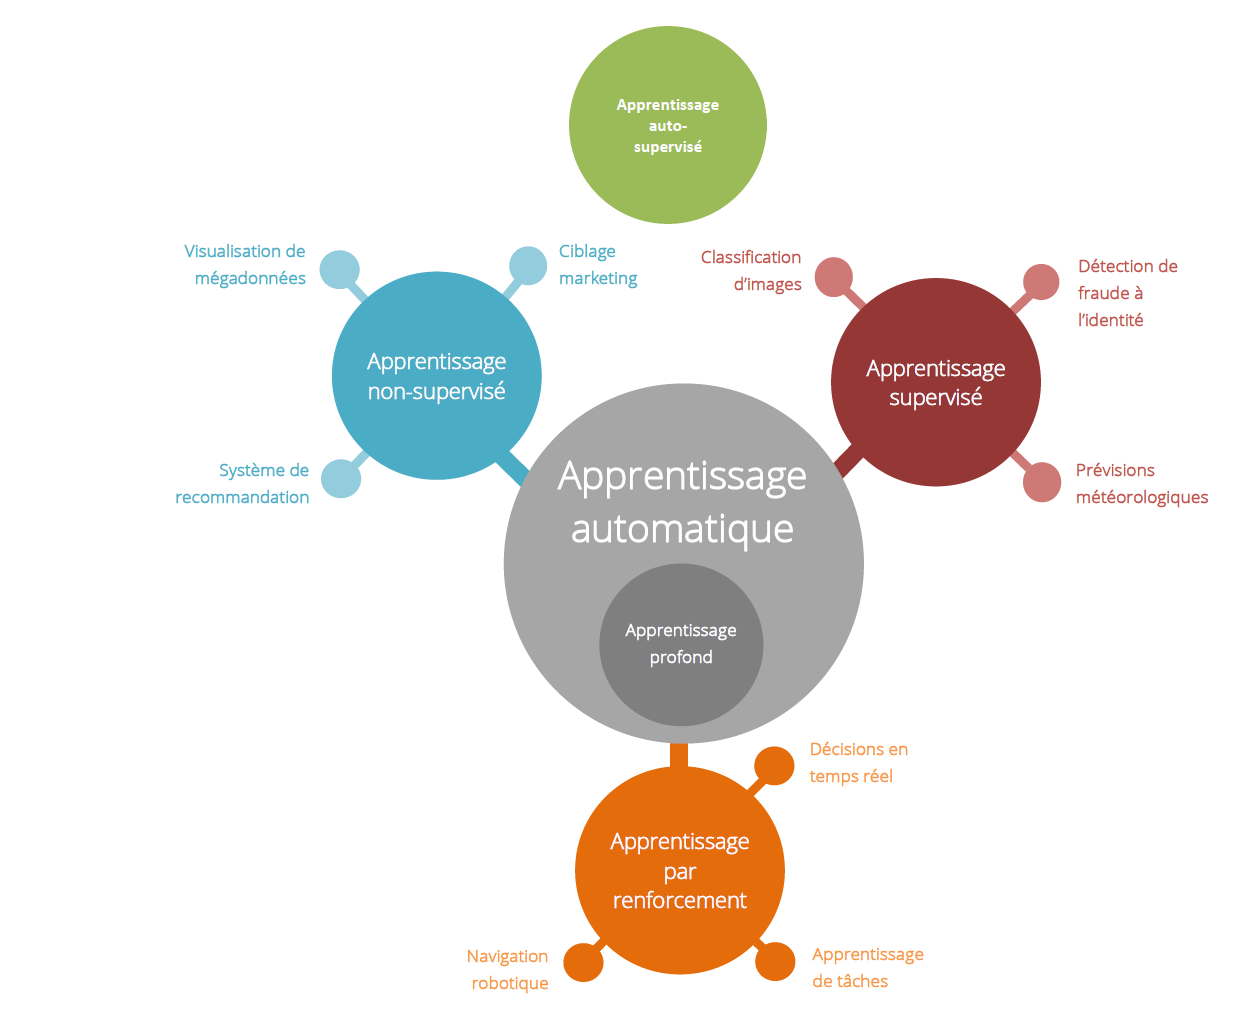
\includegraphics[width=.95\textwidth]{./Chapitre2/figures/typeApprentissage.png}
  \caption{Les différents types d'apprentissage et des exemples d'utilisation.}
  \label{fig:typeApprentissage}
\end{figure}


%Dans l'apprentissage supervisé, nous connaissons déjà les sorties souhaitées pour nos données d’entraînement. Nous avons une référence pour chaque document contenu dans les données d’entraînement et nous apprenons au système à retrouver ces références. Il y a plusieurs mots pour définir ces références. On peut parler d'étiquettes, d'annotation ou de label. Ce type d'apprentissage ne peut donc être mis en place que lorsque nous avons des données d’entraînement qui sont annotées. Cette annotation peut être effectuée soit par l'humain soit par la machine : un autre système d'apprentissage, un ensemble de règles, ... L'apprentissage supervisé peut être soit une classification, soit une régression.

Dans l'apprentissage non supervisé, %les sorties attendues pour nos données d’entraînement ne sont connues.
l'objectif du système automatique est d'inférer une caractérisation des données d'entrée : il doit capturer de lui-même les structures sous-jacentes aux données. Il n'y a pas de label pour \textit{guider} l'apprentissage. Nous spécifions le nombre de classes au système et il va essayer d'apprendre tout seul ce qui différencie les images en entrée, ici la présence ou l'absence de l'animal.

Cet apprentissage se base principalement sur deux méthodes: la méthode par partitionnement et la méthode de regroupement. Pour le partitionnement, on va chercher à diviser les entrées en un nombre $k$ de partitions. Pour cela, on peut comparer la distance entre les différents échantillons d'entrée, par le calcul d'une distance euclidienne par exemple. Le regroupement, appelé clustering en anglais, va chercher à minimiser l'inertie intra-classe, c'est-à-dire les distances entre les échantillons d'une même classe. Elle va en même temps chercher à maximiser l'inertie inter-classe, c'est-à-dire les distances entre les centres de chaque classes. %L'apprentissage non supervisé peut également servir à prédire une régression.

Un nouveau type d'apprentissage est de plus en plus utilisé depuis ces trois dernières années, notamment dans le domaine de traitement des langages naturels (TALN). On l'appelle apprentissage auto-supervisé, self supervised learning en anglais (SSL). Comme pour l'apprentissage non-supervisé, il s'agit d'un apprentissage où l'on n'a pas de références pour nos données d'apprentissage. Pour compenser leur absence, il y a plusieurs méthodes qui peuvent être utilisées. Par exemple on peut prendre une très grande masse de données et on en cache une partie. Le système devra alors retrouver les parties cachées à partir des parties disponibles. On peut également demander au système d'apprendre à prédire la suite des données. Ainsi le système crée à la volée des étiquettes qui lui permettront d'apprendre. Il s'agit en fait de mélanger les avantages de l'apprentissage supervisé et non-supervisé.
%Cette technique est utilisée par exemple dans la traduction de texte, où l'on apprend à représenter deux langues différentes puis en comparant ces deux représentations. On est ainsi capable de passer d'une langue A à une langue B sans avoir fourni au système des traductions d'un document de la langue A vers la langue B.

L'apprentissage par renforcement consiste à laisser le système inférer ses propres décisions et le récompenser positivement ou négativement en fonction de sa réponse. Le système va alors chercher, en répétant les expériences, la meilleure stratégie qui maximise la somme des récompenses au cours du temps. Cet apprentissage est très utilisé dans les jeux vidéos ou de société, où la récompense peut se traduire par la victoire ou la défaite du système par exemple. On peut citer AlphaZéro~\cite{Silver2018}, un système automatique qui a battu les meilleurs systèmes automatiques ayant eux-même battu les champions du monde humains de Go, de shogi et d'échecs.

Il existe de nombreux algorithmes permettant l'apprentissage de ces systèmes, que la tâche soit de nature supervisée, non-supervisé ou auto-supervisé.

\section{Quelques familles d'apprentissage automatique}
Dans le contexte de la reconnaissance d'émotion, de nombreuses méthodes d'apprentissage automatique sont utilisées, que ce soit pour faire de la classification lorsque l'on considère une émotion comme discrète ou de la régression quand on considère une émotion comme continue.
Dans les sections suivantes, nous détaillerons certaines d'entre elles.

\subsection{k-moyennes et k-plus proches voisins}
\textcolor{red}{a revoir, pas de corrections encore}
Les k-moyennes~\cite{Lloyd1982}, appelé k-means en anglais, et les k-plus proches voisins~\cite{Fix1951,Cover1967}, appelé k-nearest neighbors (KNN) sont des algorithmes de classification.

%\newline
% \begin{center}\fbox{\begin{minipage}{15cm}
% \begin{center}
%   \textbf{k-moyennes}
% \end{center}
Soit un ensemble de points $X_i$ avec $i=1,2,...,n$ que l'on souhaite classer en $k$ classes $C_i$ avec $i=1,2,...,k$. L’algorithme k-moyennes cherche le meilleur partitionnement afin de minimiser la distance entre les centres des classes et tous les points qui leur sont affectés.
L'ensemble des distances $D$ entre le centre $C$ de la classe $C_n$ et tous les points $X_i$ appartenant à cette classe $C_n$ est définie par l'équation~\ref{eq:quadratique}.
\begin{equation}
  D(C_n) = \sum_{X_i\epsilon C_n}   \| x_i - C \|^2
  \label{eq:quadratique}
\end{equation}
Les k premières données $X_1,...,X_k$ sont définies comme les centres $C$ des classes $C_1,...,C_k$ puis on considère la distance entre les nouvelles données $X_{k+1},...X_n$ et ces centres pour leur affecter une classe. Le centre de la classe $C$ est donc recalculé à chaque nouvelle donnée assignée à la classe.

% \begin{center}
%   \textbf{k-plus proches voisins}
% \end{center}

En ce qui concerne l'algorithme du k-plus proches voisins, il est très semblable au k-moyennes. Le centre de chaque classe est cependant fixé par l'expérimentateur et ne sera pas recalculé.
% \end{minipage}}
% \end{center}

\begin{figure}
  \centering
  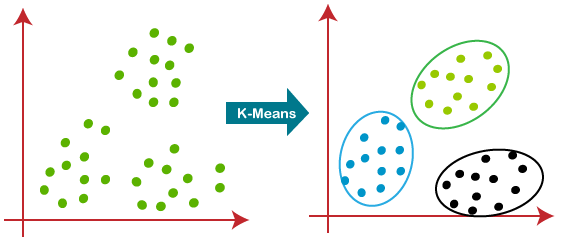
\includegraphics[width=12cm]{./Chapitre2/figures/clustering.png}
  \caption{Représentation graphique d'une classification en trois classes par un algorithme k-means.}
  \label{fig:clustering}
\end{figure}


Le k-moyennes permet de diviser les données en k groupes distincts, appelés clusters. Par exemple, dans la figure~\ref{fig:clustering}, on considère trois classes. Nous sommes donc dans un contexte d'apprentissage non supervisé.

Le k plus proches voisins est, quant à lui, un algorithme utilisé en classification supervisé : on connaît les références attendues pour les centres de classes. Le nombre de classe k est lui aussi connu et on cherche à caractériser des données en fonction de leur distance avec les données contenues dans les k classes. On décide donc de la classe d'une donnée en fonction de celle de ces plus proches voisins.

Ces deux algorithmes sont donc très dépendants de l'initialisation du système : le nombre de classes ainsi que l'ordre de présentation des données dans l'apprentissage sont des paramètres critiques.%, mais reste très utilisé~\cite{Jain2010}.

On retrouve des utilisations de ces algorithmes en NLP et en parole, par exemple avec Kamper et al. qui utilise l'algorithme du k-moyennes pour de la segmentation de parole non annotée~\cite{Kamper2017}, la classification d'actes de parole dans des jeux éducatifs~\cite{Rus2012} ou l'utilisation de l'algorithme k plus proche voisin pour la classification de texte~\cite{Zhou2015}.


% \subsection{Classification naïve bayésienne}
% La classification naïve bayésienne se base sur le théorème de Bayes~\cite{Bayes1763}. Ce théorème, qui se traduit par l'équation~\ref{eq:bayes} permet de prédire la probabilité conditionnelle de l'évènement A sachant B ($P(A|B)$) à partir des probabilités de l'évènement A ($P(A)$), l'évènement B ($P(B)$) et la probabilité de l'évènement B sachant A ($P(B|A)$).
% \begin{equation}
%     P(A|B) = \dfrac{P(B|A)xP(A)}{P(B)}
%     \label{eq:bayes}
% \end{equation}
%
% Il prend chacune des caractéristiques des données indépendamment pour faire sa classification : ce théorème suppose une indépendance entre les différentes caractéristiques, d'où son appellation de \textit{naïf}. Par exemple pour la présence d'hippopotame dans un zoo, la présence d'un bassin et le nombre d'animaux possédé par le zoo ne seront pas pris en compte conjointement.
%
% Son plus grand avantage c'est qu'il nécessite relativement peu de données d'entraînement pour estimer les paramètres nécessaires à la classification, à savoir les moyennes et les variances des différentes caractéristiques. Grâce au principe d'indépendance des caractéristiques, on n'a pas besoin de calculer la covariance entre ces dernières. Cela permet au classifieur d'être rapide et peu coûteux en puissance de calcul lors de sa phase d'apprentissage~\cite{Hand2001}.

\subsection{Régression Linéaire}
La régression linéaire permet de catégoriser des sous-espaces en fonction de la proximité des données. %Elle est à l'origine mise en place pour des régressions mais peut également être utilisée pour des classifications.
Ce type de système apprend pour chaque classe une fonction de régression linéaire qui est optimale pour représenter les données de la classe. Son objectif est d'expliquer une variable $y$ à l'aide d'une ou plusieurs variables $x$. La régression linéaire peut être simple, représentée par une fonction affine $y=ax+b$ avec $y$ la variable à expliquer, $x$ correspondant à une caractéristique de la donnée, $a$ le coefficient associé à la caractéristique et $b$ une constante.
%Pour des données mettant en lien deux variables, par exemple prédire la présence d'un hippopotame dans un zoo.
Elle peut également être multiple, représentée par l'équation~\ref{eq:regression_lineaire} lorsque plusieurs caractéristiques des données sont prises en compte. Ici, on dispose de $n$ observations appelées $y_i$ que l'on souhaite expliquer par les caractéristiques $x_{i,j}$.

\begin{equation}
  \begin{pmatrix} y_1\\ ...\\ y_n \end{pmatrix}
=
\begin{pmatrix} x_{1,1}& ...  & x_{1,p}  \\ ...& ... & ... \\ x_{n,1}& ... & x_{n,p}  \\ \end{pmatrix}
\begin{pmatrix} a_0\\ ...\\ a_p\end{pmatrix}
+
\begin{pmatrix} b_1\\ ...\\ b_n \end{pmatrix}
  \label{eq:regression_lineaire}
\end{equation}

Par exemple pour prédire la présence d'un hippopotame dans un zoo ($y_1$), les données peuvent contenir la présence d'un zoo dans une ville ($x_{1,1}$), le nombre d'animaux qui le compose ($x_{1,2}$), la présence d'un bassin ($x_{1,3}$), ...

Afin de classer une nouvelle donnée, le système va la comparer avec les différentes courbes de régression apprises en calculant l'écart de cette donnée à ces courbes. On appelle cette méthode, l'estimateur des moindres carrés.

Cette méthode éprouvée depuis plus de deux cents ans~\cite{Gauss1809,Legendre1805,Adrain1808} est explicable et facile à mettre en place.  L'apprentissage est également très rapide. Mais elle ne fonctionne pas pour toutes les tâches et toutes les données. En effet, elle implique que les caractéristiques des données permettent d'expliquer la caractéristique recherchée. Dans notre exemple, la présence d'un bibliothèque dans la ville ($x_{1,4}$) ne permettra probablement pas de prédire la présence d'un hippopotame dans un zoo.

Cet algorithme est utilisé dans des problématiques de NLP, dans des problématiques concrètes telles que la détection de vraie ou fausse note de suicide~\cite{Pestian2010}, la classification de rapport d'accident de site de construction~\cite{Zhang2019} pour déterminer la cause des incidents en combinant différents algorithmes ou encore il était utilisé dans la reconnaissance de la parole afin de réorganiser les meilleurs hypothèses de transcription~\cite{Chotimongkol2001}.

\subsection{Machine à vecteurs de support}
%\textcolor{red}{un peu de math, ça ferait pas de mal, mais je veux pas non plus que ce soit trop long}
La méthode, appelée Support Vector Machine (SVM) en anglais~\cite{Cortes1995}, est principalement utilisée pour résoudre des tâches de classification supervisée. Elle consiste en la séparation linéaire des données projetées dans un espace en utilisant un hyperplan optimal. Cette séparation est effectuée en maximisant la marge entre les données de chaque classe : l'hyperplan optimal doit être le plus éloigné des données des différentes classes tout en les séparant.

Pour avoir des résultats pertinents il faut que les données soient linéairement séparables dans le plan de projection. Si ce n'est pas le cas, l'utilisation de différents noyaux va permettre de modifier l'espace et donc la répartition des données dans cet espace. On peut par exemple voir la projection de données 2D en 3D, permettant de rendre certaines données linéairement séparables.

%Afin de classer une nouvelle donnée, le système va donc placer cette donnée dans l'espace de représentation et situer son emplacement par rapport à l'hyperplan séparateur.
Cette méthode est très utilisée en classification, étant assez rapide à apprendre. De plus, elle est très performante lorsque l'on possède peu de données d'apprentissage.

On retrouve des utilisations de SVM dans les domaines de l'ASR, notamment couplé à d'autres algorithmes dans~\cite{Solera2007}, dans la reconnaissance d'émotion, des SVM sont utilisés dans les arbres de décisions de~\cite{Rozgic2012} pour déterminer si une phrase énoncée fait partie des quatre catégories (joie, colère, tristesse et neutre) ou encore dans la tâche de reconnaissance d'entités nommés dans la langue arabe~\cite{Benajiba2008}.

\subsection{Modèle de Markov caché et prédiction de séquence}

Le modèle de Markov caché, appelé hidden Markov model (HMM) en anglais~\cite{Rabiner1986}, est un modèle probabiliste à base d'automates. Ces automates se composent d'états qui sont reliés par des transitions, comme montré sur la figure~\ref{fig:hmm}.

\begin{figure}[h]
  \centering
  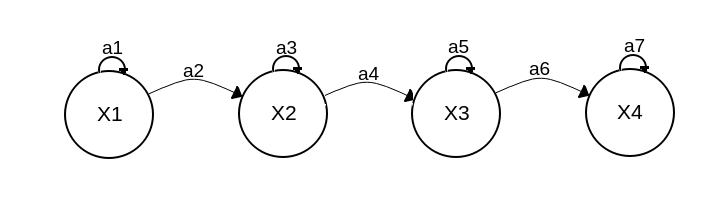
\includegraphics[width=16cm]{./Chapitre2/figures/hmm.png}
  \caption{Représentation graphique d'un modèle de Markov caché à quatre états. $X$ représente les états de l'automate, $a$ représente les transitions entre les états.}
  \label{fig:hmm}
\end{figure}


Chaque transition boucle sur lui-même et va vers l'avant et correspond à la probabilité de changer de l'état courant pour le suivant. Comme le changement d'état n'est pas obligatoire, une transition circulaire est mise en place pour boucler sur l'état courant.
Utilisé en classification principalement, en apprentissage supervisé ou non, il va considérer chaque élément de nos données d'entrée de manière séquentielle pour prédire son état final.

Les modèles de Markov cachés ont été massivement utilisés notamment en ASR, en reconnaissance d'écriture manuscrite~\cite{Hu1996}, en intelligence artificielle~\cite{Gales2008}, en traitement automatique du langage naturel~\cite{Campbell2006} ou en segmentation et regroupement de locuteurs~\cite{Ajmera2002}.

\subsection{Modèle de mélange gaussien}
Le modèle de mélange gaussien, appelé Gaussien Mixture Model (GMM) en anglais, est très souvent associé aux HMM. En effet, il permet d'associer un ensemble de densités de probabilités aux différents états, selon un mélange de lois gaussiennes. Les paramètres de ces dernières sont appris lors de la phase d'apprentissage par la maximisation de la vraisemblance. Le nombre de gaussiennes est un hyper-paramètre fixé par l'humain. Sur la figure~\ref{fig:gmm}, on peut voir un modèle à trois gaussiennes.

\begin{figure}[h]
  \centering
  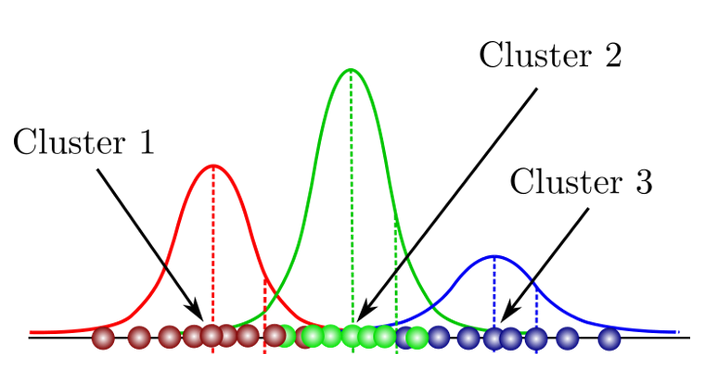
\includegraphics[width=14cm]{./Chapitre2/figures/gmm.png}
  \caption{Représentation graphique d'un modèle de mélange de trois gaussiennes.}
  \label{fig:gmm}
\end{figure}


Les GMM sont notamment utilisés dans des tâches de NLP tel que le résumé automatique de texte~\cite{Fattah2009} ou encore pour la vérification de locuteur~\cite{Baker2005}. Couplés aux HMM, ils ont longtemps été les systèmes à l'état de l'art majoritaires pour la reconnaissance de la parole, jusque dans les années 2010~\cite{Hinton2012}. Aujourd'hui, les réseaux de neurones sont de plus en plus utilisés pour améliorer notamment la reconnaissance de la parole.

\subsection{Réseau de neurones}
Les réseaux de neurones ont été conçus en s'inspirant du fonctionnement du cerveau humain. Ils sont composés d'une succession de neurones qui sont interconnectés entre eux pouvant ainsi propager des signaux.
Afin de mieux comprendre leur fonctionnement, il est intéressant de les mettre en relation avec la biologie du système nerveux de l'homme.

\begin{figure}
  \centering
  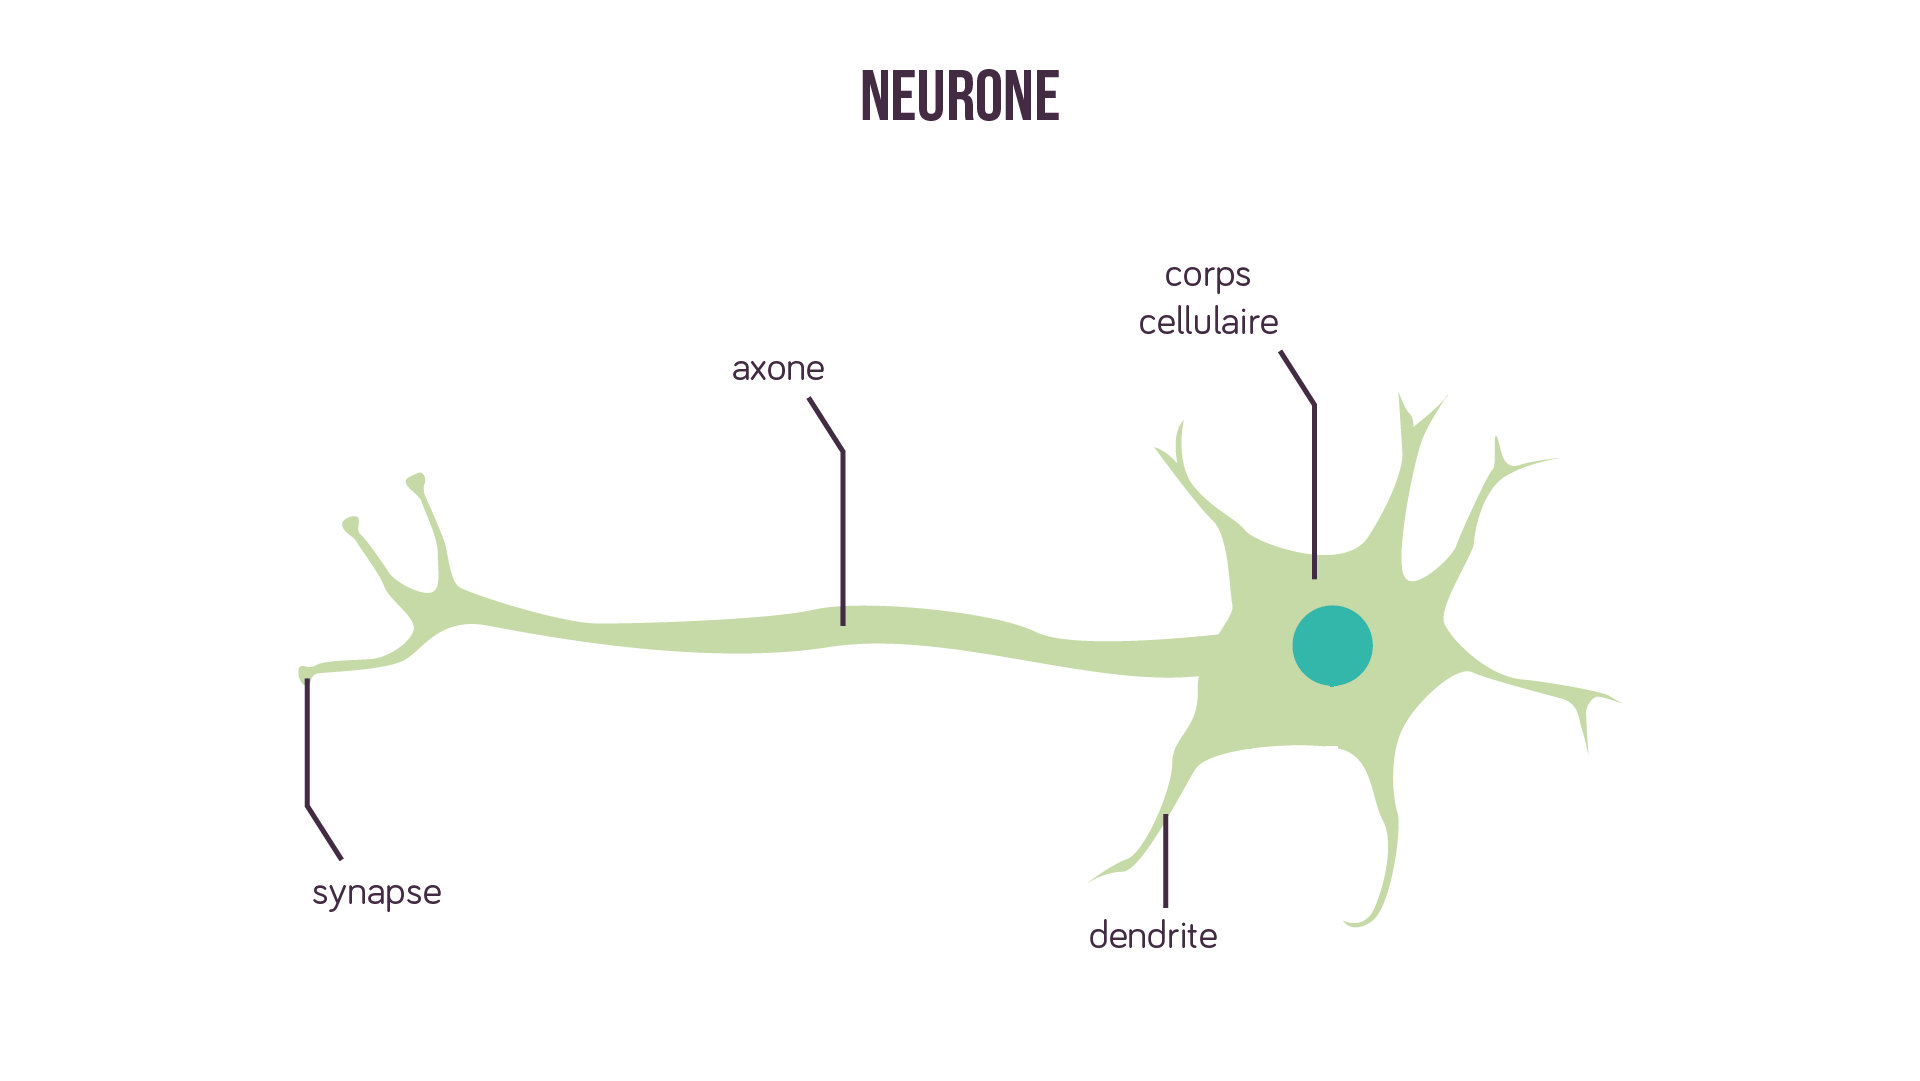
\includegraphics[width=10cm]{./Chapitre2/figures/neuroneBio.png}
  \caption{Représentation schématique d'un neurone biologique. Illustration issue de shorturl.at/uvL34 .}
  \label{fig:neuroneBio}
\end{figure}

Au début du XXe siècle, les avancées de la biologie ont permis de mettre en lumière les méthodes de fonctionnement de notre système nerveux~\cite{Cajal1906}. On définit alors les neurones en tant que corps cellulaire muni d’un axone et de dendrites. Cette cellule, illustrée dans la figure~\ref{fig:neuroneBio} est traversée par des influx nerveux de type électrique, qui entrent par les dendrites et ressort par les synapses de son axone. Chaque neurone peut être relié à un ou plusieurs neurones, que ce soit en entrée ou en sortie.
C'est en 1943 que Warren Sturgis McCulloch et Walter Pitts proposent une représentation mathématique des neurones~\cite{McCulloch1943}, que l'on appelle neurone logique dans la suite de ce document. Ils définissent plusieurs principes :
\begin{itemize}
  \item un neurone biologique peut être représenté par un neurone logique,
  \item les entrées du neurone logique sont comparables aux dendrites,
  \item le neurone logique possède une seule sortie qui représente l'axone,
  \item les connexions entre les neurones se font par le clonage de la sortie en autant de liens qu'il y a de prochains neurones, représentant les connexions synaptiques,
  \item la fonction d'activation correspond à une prise de décision au niveau du neurone logique qui représente un potentiel d'activation : le neurone biologique émet un influx nerveux ou non.
\end{itemize}
C'est à partir de ces règles que les réseaux de neurones % profonds, appelé deep neural network (DNN)
vont être définis.

\section{Réseau de neurones profonds}
Les réseaux de neurones profonds sont de nos jours de plus en plus utilisés. Pourtant, ils ne sont pas récents : le premier algorithme d'apprentissage utilisant un réseau de neurones a plus de 50 ans. Il s'agit du perceptron de Frank Rosenblatt~\cite{Rosenblatt1957}.

\subsection{Du perceptron au multicouche}
\begin{figure}[h]
  \centering
  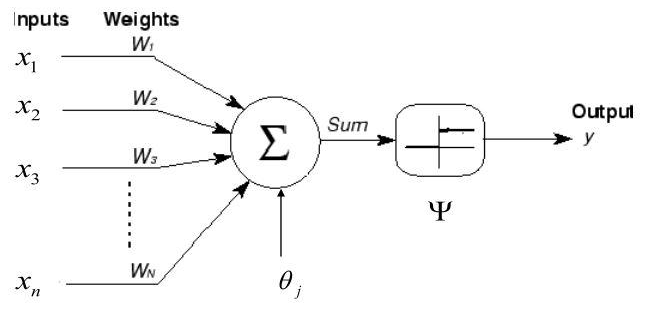
\includegraphics[width=11cm]{./Chapitre2/figures/perceptron.png}
  \caption{Représentation schématique d'un perceptron. $x_i$ correspond aux entrées, les $W_i$ correspondent aux poids associés à chacune des entrées $x_i$, $\psi$ formalise le biais. Une fois sommée, la valeur est passée dans une fonction d'activation $\phi$ pour déterminer la valeur de sortie $y$. Dans le schéma la fonction d'activation correspond à un simple signal échelon.}
  \label{fig:perceptron}
\end{figure}

Le perceptron, schématisé dans la figure~\ref{fig:perceptron}, est un modèle qui permet de discriminer les données en deux classes. Il s'agit donc d'un modèle qui permet de faire de la classification et de la régression de manière supervisée. Ce modèle binaire utilise un neurone pour l'apprentissage et la prédiction de la classe de chaque document. Un document est défini par un nombre $n$ de caractéristiques, chacune d'entre elles étant considérées comme une entrée du perceptron.

Lors de l'apprentissage, des poids $w_i$, initialisés de façon aléatoire, sont mis à jour pour chacune des entrées. Cette mise à jour est effectuée en fonction du taux d'apprentissage, appelé learning rate en anglais, afin de retrouver les étiquettes déjà connues des données d'apprentissage. En plus du poids, le biais est également défini lors de l'apprentissage. Il correspond à un unique poids qui sera utilisé pour la prédiction des étiquettes des données. Les entrées sont ainsi agrégées en les pondérant selon leur poids. La fonction d'agrégation est explicitée par l'équation~\ref{eq:aggregation}, où $x_i$ correspond à l'entrée i, $w_i$ correspond au poids associé à l'entrée i et $b$ correspond au biais.
\begin{equation}
  z = \sum_{i=1}^{n}(w_i*x_i) - b
  \label{eq:aggregation}
\end{equation}

Une fonction d'activation est ensuite appliquée. Dans le cas du perceptron de Rosenblatt, soit le tout premier perceptron, la fonction d'activation est définie par une fonction échelon qui prend une valeur de 0 si $z$ est inférieur ou égal à 0 et une valeur de 1 s'il est strictement supérieur à 0.

Le perceptron est une architecture très simple qui est de moins en moins utilisée. En effet, elle permet de résoudre uniquement des problèmes binaires linéairement séparables. Le perceptron multicouche est notamment capable de palier à ces inconvénients.

\begin{figure}
  \centering
  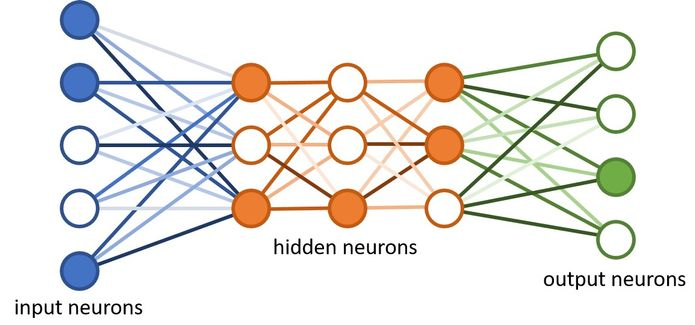
\includegraphics[width=8cm]{./Chapitre2/figures/perceptronMLP.png}
  \caption{Représentation schématique d'un perceptron multi-couche. Les neurones bleu correspondent à la couche d'entrée, les neurones oranges définissent plusieurs couches cachées et les neurones verts correspondent à la couche de sortie.}
  \label{fig:perceptronMLP}
\end{figure}

Ce dernier, appelé multilayer perceptron (MLP) en anglais, assemble plusieurs neurones entre eux comme illustré dans la figure~\ref{fig:perceptronMLP}. Un ou plusieurs neurones sont assemblés les uns à la suite des autres. On a forcément une couche de neurones (ou un neurone seul) en entrée, qui reçoit les caractéristiques de chaque donnée et une couche de neurones (ou un neurone seul) en sortie qui prend la décision finale. Entre les deux, on trouve éventuellement des couches intermédiaires dites cachées, qui vont prendre en entrées les sorties de la couche précédente (soit la couche d'entrée, soit une autre couche cachée) et en sortie la couche suivante (soit une autre couche cachée soit la couche de sortie).

Les informations vont donc être propagées de la couche d'entrée à la couche de sortie. On appelle cette propagation, propagation directe avant, ou forward propagation en anglais. Le nombre de couches et le nombre de neurones par couche doivent être définis par l'utilisateur afin d'être en adéquation avec la tâche visée. Par exemple, le nombre de neurones de sortie permet de définir le nombre de classes dans une classification.

\begin{figure}
  \centering
  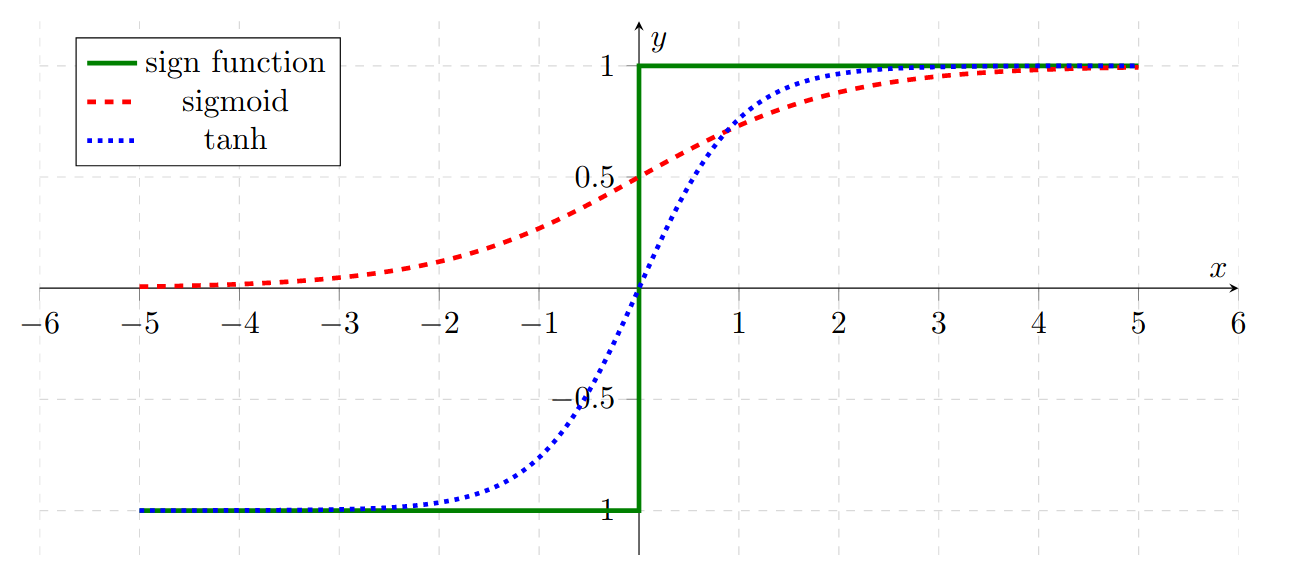
\includegraphics[width=11cm]{./Chapitre2/figures/activation.png}
  \caption{Représentation graphique de trois fonctions d'activation : la fonction non linéaire, sigmoide et tanh. Illustration provenant de~\cite{Thoma2014}.}
  \label{fig:activation}
\end{figure}


Il existe plusieurs fonctions d'activation qui peuvent être utilisées. On utilise le plus souvent, en plus de la fonction échelon, les fonctions sigmoïde et tangente hyperbolique qui sont décrites dans la figure~\ref{fig:activation}. La fonction sigmoïde est définie par l'équation~\ref{eq:sigmoide} et la fonction tangente hyperbolique, abrégé tanh, est définie par l'équation~\ref{eq:tangente}. Le choix de ces différentes fonctions influence le résultat de la classification ou de la régression.

\begin{equation}
  f(x) = \frac{1}{1+ e^{-x}}
  \label{eq:sigmoide}
\end{equation}

\begin{equation}
  tanh(x) = \frac{1-e^{-2x}}{1+e^{-2x}}
  \label{eq:tangente}
\end{equation}

Le perceptron multicouche correspond à l'une des premières architectures dites profondes. En effet, il est constitué d'au moins deux couches. Les chercheurs admettent que le nombre de couches est croissant en fonction de la difficulté de la tâche à accomplir~\cite{Goodfellow2016}. Mais plus le système est complexe (plus il a de couches et de neurones par couche), plus la phase d'apprentissage sera compliquée car elle demandera beaucoup de données et de puissance de calcul.
En partant du principe de couches successives, de nombreuses architectures particulières ont vu le jour. Les architectures utilisées dans le Speech Emotion Recognition sont décrites dans le prochain chapitre. Mais avant d'explorer les architectures, nous allons nous intéresser aux méthodes d'apprentissages.

\subsection{Algorithme d'apprentissage}
L'apprentissage des réseaux de neurones correspond à apprendre différents paramètres, dont notamment des poids et des biais. Il est important de dissocier les paramètres des hyper-paramètres. Ces derniers sont définis au préalable de l'apprentissage, par l'évaluateur. Par exemple pour un réseau de neurones, on retrouve comme hyper-paramètres le nombre de couches, le nombre de neurones par couches, le taux d'apprentissage. Il est également essentiel de définir la présentation des données, quelle soit à l'unité, soit une par une ou en lot (batch). La présentation par lot permet généralement d'avoir des systèmes ayant un pouvoir de généralisation plus grand, puisqu'on laisse le système voir plusieurs données avant d'actualiser ces paramètres. De même le nombre d'époques, soit le nombre de fois que le système voit les données, est un hyper-paramètre essentiel dans la configuration de l'apprentissage.

En apprenant les paramètres, le système peut alors s'en servir pour prédire une référence, que ce soit une classe (classification) ou une valeur numérique (régression). Cette prédiction est obtenue à partir d'un ensemble de caractéristiques, appelés features en anglais, d'une donnée. Ces paramètres sont mis à jour au fur et à mesure de la présentation des données d'apprentissage au réseau, afin de trouver des paramètres optimaux qui permettent de maximiser les bonnes prédictions. Il est donc essentiel de mettre en place cet apprentissage sur des données cohérentes avec la tâche visée.

Afin de réaliser cette phase d'apprentissage, il est nécessaire de définir une fonction de coût% et le gradient
. La fonction de coût correspond à une fonction que l'apprentissage va chercher à minimiser et qui correspond à une distance entre les valeurs prédites par le système et les valeurs attendues (les références). %Le gradient correspond au vecteur regroupant toutes les dérivées partielles de la fonction de coût.

\subsubsection{Fonction de coût}
Il existe de nombreuses fonctions de coût qui permettent de calculer l'écart entre les valeurs prédites et les valeurs de références. %Grâce à des méthodes mettant en jeu le gradient, le rôle de l'apprentissage automatique sera de minimiser l'écart entre ces deux valeurs, afin de se rapprocher le plus possible des références et donc d'avoir un système performant.
Par exemple l'erreur quadratique moyenne, appelée mean square error (MSE) en anglais, est une fonction de coût très utilisée qui a pour avantage d'être simple et rapide à calculer. Elle consiste à calculer la différence quadratique entre l'observation, notée $O$, et la prédiction, notée $p$, d'une donnée selon l'équation~\ref{eq:mse} :
\begin{equation}
  MSE = \frac{1}{n}\sum_{i=1}^{n}(O-p)^2
  \label{eq:mse}
\end{equation}
$n$ correspond aux nombres d'observation lors des différentes époques. Parmi les fonctions de coût les plus utilisées, on peut notamment citer l'entropie croisée~\cite{Stemmer2002}, la Classification Temporelle Connexionniste (CTC)~\cite{Graves2006} ou encore la somme des carrés des résidus (SCR). C'est donc cette fonction de coût que l'on va dériver pour récupérer la valeur du gradient, que l'on utilise pour apprendre un système automatique.
%\textcolor{red}{a part pour etre exhaustif, expliciter les fonctions de cout ne me semble pas pertinent, puisqu'on ne les utilise pas par la suite.}

% \subsubsection{Rétropropagation du gradient}
% Lors de la phase d'apprentissage, le système va chercher à minimiser les erreurs de prédiction. Pour ce faire, nous allons chercher la meilleure configuration de poids possible. L'algorithme de rétropropagation du gradient (backpropagation en anglais) va nous permettre de calculer l'erreur $E$ pour chacun des neurones en partant de la dernière couche et en remontant jusqu'à la première. Cette méthode, introduite par Rumelhart et al.~\cite{Rumelhart1986}, se divise en deux parties. Tout d'abord on calcule l'erreur globale $\delta E$ en comparant les prédictions et les références, en utilisant la fonction de coût. Les prédictions sont obtenues en soumettant le système à une donnée et elles sont directement impactées par la matrice de poids $W$ des neurones de chaque couche. Puis on va propager la dérivée partielle de l'erreur $\frac{\delta E}{\delta W}$ de couche en couche en fonction des poids du réseau $W$, de la dernière jusqu'à la première.
%
% Ainsi, la propagation des erreurs va permettre de modifier les poids associés à chaque neurone, en prenant en compte leur part dans l'erreur calculée. En fonction de la part de "responsabilité" d'un neurone dans l'erreur, son poids associé $W'$ va être plus ou moins modifié pour que le neurone devienne plus activateur ou plus inhibiteur selon l'équation~\ref{eq:poids}.
%
% \begin{equation}
%   W' = W - \lambda \frac{\delta E}{\delta W}
%   \label{eq:poids}
% \end{equation}
%
% $\lambda$ correspond au taux d'apprentissage, ou learning rate, qui permet de contrôler l'intensité de la variation entre deux mises à jour. Un taux faible équivaut à des variations faibles rendant l’apprentissage lent mais qui peut garantir une certaine stabilité. L'impact de ce taux sera détaillé dans la prochaine section.
%
% \subsubsection{Descente de gradient}
% La descente du gradient est utilisée pour apprendre à minimiser la fonction de coût $C$. Comme nous l'avons défini plus tôt, le gradient correspond à un vecteur regroupant les dérivées partielles de la fonction de coût. Si on se place dans un système à un seul paramètre, le gradient correspond au coefficient directeur de la droite de régression linéaire. %Comme il y a autant de dérivées partielles que de variables, le calcul de la valeur minimisant la fonction de coût demande trop de combinaison à calculer. On utilise donc un algorithme de descente de gradient qui revient à effectuer une approximation du minimum de la fonction de coût.
%
% La méthode de descente du gradient consiste à mettre en place une variation des paramètres de la fonction de coût par des itérations successives. Ce pas est défini par le taux d'apprentissage noté $\lambda$. Ce taux permet de faire varier les paramètres de la fonction de coût lors des itérations. Pour chaque paramètres $\theta_1$, $\theta_2$, $\theta_n$ de la fonction de coût, la descente de gradient se définit par l'équation~\ref{eq:descente} :
% \begin{equation}
%   x_{n+1} = x_n - \lambda (\dfrac{\delta C(x)}{\delta x_i})
%   \label{eq:descente}
% \end{equation}
%
% \begin{figure}[h]
  \centering
  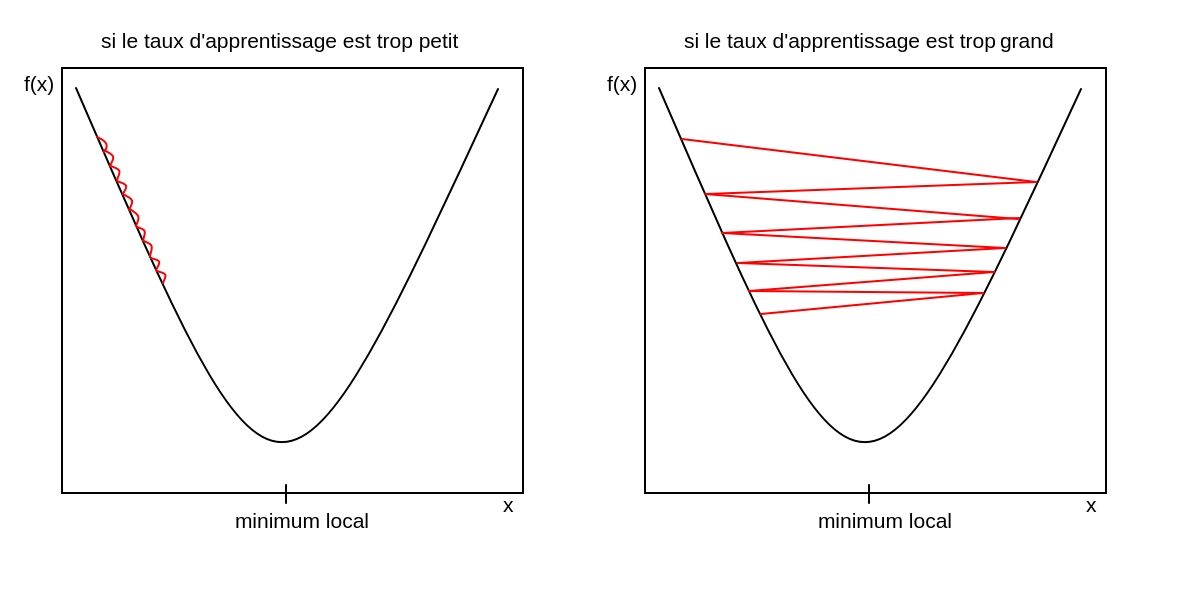
\includegraphics[width=.95\textwidth]{./Chapitre2/figures/tauxApprentissage.png}
  \caption{Exemple de la descente de gradient dans le cas d'un taux d'apprentissage soit trop petit, soit trop grand. L'apprentissage est composé de dix mises à jour des poids.}
  \label{fig:tauxApprentissage}
\end{figure}

%
% Cet algorithme n'est pas exempt d'inconvénients. En effet, selon la fonction de coût considérée, il est possible qu'il existe plusieurs minimums mais qui ne correspondent pas au minimal global. On appelle ces zones des minima locaux : converger dans une de ces zones signifie une suboptimalité du réseau de neurones. En fonction du taux d'apprentissage utilisé, il est donc possible que l'algorithme de descente de gradient converge vers un minimum local à la place du minimum global.
%
% Comme illustré dans la figure~\ref{fig:tauxApprentissage}, plus le taux d'apprentissage est petit, le temps d'apprentissage est long. Cependant si le taux d'apprentissage est trop grand, il est tout à fait possible de ne jamais converger vers un minima. L'initialisation de ce taux est donc très important.
%
% Cette descente de gradient connaît deux principales variantes : la descente de gradient stochastique et la descente de gradient par lot (batch en anglais). La descente de gradient stochastique va mettre a jour les paramètres après chacun des échantillons des données d'apprentissage vus lors de l'apprentissage. La descente de gradient par lot va mettre à jour les paramètres après avoir vu tous les échantillons. La mise à jour se fait en considérant la moyenne des gradients. La méthode de mini-batch correspond quant à elle à une méthode inspirée des deux variantes : la mise à jour des paramètres se fait après avoir vu un ensemble d'échantillons.
% % Cette mise à jour est définie par l'équation~\ref{eq:SGD} où $w$ correspond aux poids, $\lambda$ au taux d'apprentissage et $C$ à la fonction de coût.
% % \begin{equation}
% %   w_{t+1} = w_{t} - \lambda\hat{\nabla}_{w}{C(w_{t})}
% %   \label{eq:SGD}
% % \end{equation}
% Dans les systèmes neuronaux actuels, cette troisième solution hybride est la plus utilisée puisqu'elle permet de diminuer le temps d'apprentissage tout en garantissant de bonnes performances.
%
%
% \subsubsection{Algorithme d'optimisation du gradient}
% Afin de rendre nos réseaux plus performants mais également répondre à des problématiques de coût matériel et temporel, on utilise des algorithmes d'optimisation du gradient. Ces algorithmes ont été développés dans un premier temps pour répondre à la problématique des minimaux locaux, mais ils sont aujourd'hui notamment utilisés pour diminuer le temps d'apprentissage sur des configurations matérielles limitées.
% Les algorithmes d'optimisation adaptatifs que sont AdaGrad et Adam sont les plus utilisés de nos jours. Ces derniers ont pour objectifs de changer dynamiquement les paramètres du système lors de l'apprentissage.
%
% \paragraph{AdaGrad}
% AdaGrad, notation pour Adaptive gradient, a été introduit par Duchi et al.~\cite{Duchi2011}. Cette méthode d'optimisation de gradient permet d'adapter dynamiquement le taux d'apprentissage. La variation du taux d'apprentissage est proportionnelle à l'historique des mises à jour des paramètres du réseau de neurones. Ainsi, si un paramètre est peu fréquent, la mise à jour sera plus important et inversement s'il est moins fréquent. Ce nouveau taux d'apprentissage est défini à chaque époque par l'équation~\ref{eq:adagrad}.
% \begin{equation}
%   \theta_{t+1, i} = \theta_{t, i} - \frac{\lambda}{\sqrt{G_{t, ii} + \epsilon}}g_{t, i}
%   \label{eq:adagrad}
% \end{equation}
% $\theta$ correspond au paramètre en cours de mise à jour, $\lambda$ au taux d'apprentissage. $G$ représente l'historique accumulé lors des précédentes époques. On ajoute un coefficient $\epsilon$ pour éviter la division par zéro, dans le cas où l'historique du gradient est égal à zéro. AdaGrad permet donc de faire évoluer le taux d'apprentissage automatiquement, rendant l'apprentissage plus efficace et robuste.
%
% Cependant l'algorithme tend à abaisser le taux d'apprentissage de façon drastique en fin d'apprentissage, ce qui stoppe l'apprentissage du système. Pour remédier à ce problème, une autre méthode est proposée.
%
% \paragraph{Rprop et RMSprop}
% Rprop, abréviation de resilient backpropagation, introduit par Riedmiller et al.~\cite{Riedmiller1993} en 1993, est un algorithme d'optimisation de gradient par lot entier. Son objectif est de palier au problème des trop grandes variations du gradient. Quand les gradients sont très grands et que d'autres gradients sont très petits, il est alors compliqué de déterminer un taux d'apprentissage pertinent. Cela peut être du à une disparité dans les données ou une tâche compliquée par exemple. Cette méthode propose d'utiliser uniquement le signe des gradients. Ainsi on garantit une évolution de même ordre pour toutes les mises à jour des poids. Cette évolution tend à éviter les plateaux et les minimums locaux, pour optimiser la convergence du système neuronal. Cet algorithme peut être divisé en trois étapes :
% \begin{itemize}
%   \item On considère le signe des deux derniers gradients et on les compare.
%   \item S'ils sont du même signe et donc qu'ils vont dans la même direction, le prochain pas d'apprentissage est multiplié par $1.2$ pour aller plus vite dans la bonne direction. S'ils sont de signes contraires, alors notre ancien pas était trop important, on le diminue donc en multipliant par $0.5$~\cite{Riedmiller1993}.
%   \item On s'arrête quand on atteint une taille de pas défini par l'utilisateur en amont, en fonction des données.
% \end{itemize}
%
% Le problème de cet algorithme, c'est qu'il n'est pas performant pour une considération en mini-batch. RMSprop (Root Mean Square propagation), proposé par Tieleman et Hinton~\cite{Tieleman2012}, a pour objectif de palier à ce problème. Pour cela, on va conserver la moyenne glissante des carrés des gradients pour tous les poids. Ainsi on adapte le taux d'apprentissage avec la moyenne glissante et non avec la moyenne de chaque mini-batch. La moyenne glissante est calculée selon l'équation~\ref{eq:movingAVG} à un instant $t$ où $E[g^{2}]$ correspond à la moyenne glissante des gradients $g$ et $\gamma$ à une constante du momentum souvent fixée à 0.9~\cite{Tieleman2012}.
%
% \begin{equation}
%   E\left[g^{2}\right]_{t} = \gamma E\left[g^{2}\right]_{t-1} + \left(1 - \gamma\right) g^{2}_{t}
%   \label{eq:movingAVG}
% \end{equation}
%
% Une fois la moyenne glissante calculée, on peut définir le nouveau taux d'apprentissage selon l'équation~\ref{eq:RMSprop}, où on retrouve la moyenne glissante $E[g^{2}]$, le taux d'apprentissage $\lambda$ et $\epsilon$ une constante faible pour éviter la division par zéro.
% \begin{equation}
%   \theta_{t+1} = \theta_{t} - \frac{\lambda}{\sqrt{E\left[g^{2}\right]_{t} + \epsilon}}g_{t}
%   \label{eq:RMSprop}
% \end{equation}
%
% Cet algorithme permet de remédier au problème d'AdaGrad en accumulant les carrées des gradients et qu'il n'y a pas de normalisation de ce dernier, le taux d'apprentissage subit des variations drastiques en fin d'apprentissage. Mais un autre algorithme plus récent est aujourd'hui beaucoup plus utilisé.
%
% \paragraph{Adam}
% L'algorithme Adam (Adaptative Moment Estimation), introduit par Kingma et al.~\cite{Kingma2015}, est l'une des méthodes les plus utilisées actuellement. Il combine les avantages des précédentes méthodes : elle corrige l'inconvénient de l'accumulation des gradients quadratiques (AdaGrad) et elle est appropriée pour les gradients bruités ou variant fortement (RMSprop). Le calcul des poids du réseau à l'instant $t$ est réalisé selon l'équation~\ref{eq:Adam}.
% \begin{equation}
%   w_{t} = w_{t-1} - \lambda\frac{\hat{m}_{t}}{\sqrt{\hat{v}_{t}} + \epsilon}
%   \label{eq:Adam}
% \end{equation}
%
% $w$ est une matrice qui correspond aux poids à l'itération t, $\lambda$ au taux d'apprentissage, $\hat{m}$ l'accumulation des gradients dont sa correction est défini par l'équation~\ref{eq:m} et $\hat{v}$ l'accumulation des carrés des gradients dont sa correction est défini par l'équation~\ref{eq:v}. On utilise la correction de $m$ et $v$, noté $\hat{m}$ et $\hat{v}$, pour palier au biais dénoté par les auteurs~\cite{Kingma2015}, lorsque les vecteurs sont proches de $0$.
%
% \begin{equation}
%   \hat{m}_{t} = \frac{\beta_{1}m_{t-1} + (1-\beta_{1})g_{t}}{1-\beta^{t}_{1}}
%   \label{eq:m}
% \end{equation}
%
% \begin{equation}
%   \hat{v}_{t} = \frac{\beta_{2}v_{t-1} + (1-\beta_{2})g_{t}^{2}}{1-\beta^{t}_{2}}
%   \label{eq:v}
% \end{equation}
%
% Les paramètres $\beta_{1}$ et $\beta_{2}$ correspondent à des taux de décroissance compris entre $0$ et $1$. Ils sont généralement fixés à respectivement $0.9$ et $0.999$~\cite{Kingma2015}. On utilise toujours un $\epsilon$ faible pour éviter une division par zéro.
%
% Des variantes de cet algorithme ont été publiées, dont AdaDelta~\cite{Zeiler2012} ou NAdam~\cite{Dozat2016} mais Adam reste l'algorithme majoritairement utilisé grâce à ses bonnes performances et la réduction significative apportée au temps d'apprentissage.
%
% Les algorithmes d'optimisation du gradient ne sont pas les seuls leviers permettant une meilleure performance du système. En effet, tous ces algorithmes sont fortement influencés par l’initialisation des poids effectuée en début d'apprentissage.

\subsection{L'initialisation et ses enjeux}
Comme nous l'avons dit précédemment, l'initialisation des poids d'un modèle neuronal est très importante pour garantir de bonnes performances et une convergence rapide du système. Nous allons détailler dans cette section, quelques unes des techniques d'initialisation des poids utilisées de nos jours.


\subsubsection{Initialisation aléatoire}
La plus simple de ces initialisations est d’utiliser des valeurs de poids tirées au hasard comprises entre -1 et 1. Facile à mettre en place, elle ne favorise pas un apprentissage efficace. Cependant elle est toujours utilisée de nos jours pour sa rapidité d'exécution et sa performance toute relative. En fonction de la loi de probabilité utilisée, elle peut conduire à des performances satisfaisantes voir optimales des réseaux de neurones. Ce tirage aléatoire suit généralement des distributions définies par des lois statistiques telles que la loi normale ou la loi de poisson par exemple.

La méthode de Xavier, introduite par Glorot et Bengio~\cite{Glorot2010}, garde le principe de l'initialisation aléatoire tout en la contraignant. En effet, elle considère des poids aléatoires mais dont la moyenne est égale à $0$ et dont la variance doit être constante entre les couches neuronales.

En pratique, il faut effectuer plusieurs apprentissages avec des initialisations différentes, pour trouver plusieurs minima et retenir le système le plus performant. Cette stratégie permet également de quantifier l'impact de l'initialisation sur le système considéré. Il est néanmoins très difficile voir impossible de s'assurer que le minimum trouvé correspond au minimum global. En effet, Bishop démontre dans son livre~\cite{Bishop2006} que pour un systèmes à $n$ neurones, le nombre de minima locaux est de $2^n n!$.

Il existe d'autres méthodes qui ne s'appuient pas sur une initialisation aléatoire, mais sur un apprentissage préalable de poids pour le réseau considéré.

\subsubsection{Pré-apprentissage}
La méthode de transfert d'apprentissage (transfer learning en anglais) est une méthode de plus en plus utilisée~\cite{Pan2010,Weiss2016} qui propose que les poids des neurones soient appris en amont de l'apprentissage du système sur la tâche visée. Ce premier apprentissage se fait sur des données plus nombreuses et ont pour but de mieux représenter les données utilisées, sur une tâche proche de celle visée. Par exemple, pour effectuer de la reconnaissance d'entités nommées, on va dans un premier temps apprendre à reconnaître automatiquement la parole. Donc on va utiliser les poids appris pour faire de la reconnaissance automatique de la parole pour initialiser les poids d'un système de reconnaissance des entités nommées par exemple. Comme les entités nommées sont formées de mots, ces deux tâches sont différentes mais proches. Ainsi, nous pouvons initialiser notre système avec des poids qui permettent de reconnaître des mots avant de reconnaître des entités nommées.

Comme nous avons effectué un apprentissage en amont, les poids des neurones ont pu se stabiliser une première fois, afin d'atteindre une première représentation intermédiaire. Les avantages de cette technique sont multiples. Dans un premier temps, elle permet d’accélérer la convergence d'un système. Comme nous avons déjà des poids stables et considérés comme assez proches de leur optimum, on se libère de toute une partie de la phase d'apprentissage pendant laquelle le système cherche une représentation correcte des données. Dans un second temps, l'utilisation de ces poids aide à palier au manque de données concernant la tâche visée. Puisque les poids ont été initialisés sur d'autres données, proche de celle de la tâche considérée, le pré-apprentissage peut être considéré comme une méthode d'augmentation de données.

Elle n'a pas que des avantages. En effet, il faut posséder d'autres données proche de celles de notre tâche. Il faut également que la tâche visée par le pré-apprentissage soit cohérente avec la tâche courante. En tant qu'observateur humain, on peut définir deux tâches comme étant proches alors que le réseau de neurones ne les considère pas en tant que tel, ce qu'on appelle du transfert d'apprentissage négatif. De même, l'utilisation de ces poids pré-appris peut aboutir à des situations de sur-apprentissage, dont nous parlerons dans une prochaine section.

% \subsubsection{Impact de l'initialisation}
% Afin de se rendre compte facilement de l'impact de l’initialisation sur des systèmes d'apprentissage, on peut utiliser un algorithme d'apprentissage simple : le k-moyennes. Par définition, ce dernier est défini en fonction du nombre de classes k visées et de l'ordre de visualisation des données. Comme les k premières données sont considérées comme les premières données de chaque classe, il est assez intuitif de voir l'impact de cet ordre sur la classification finale des données. Un exemple est proposé sur la figure~\ref{fig:kmeans}. Deux classifications très différentes sont observées sur les mêmes données en fonction de l’initialisation du premier centroide.
% \begin{figure}[ht]
  \centering
  \begin{subfigure}{.49\textwidth}
    \centering
    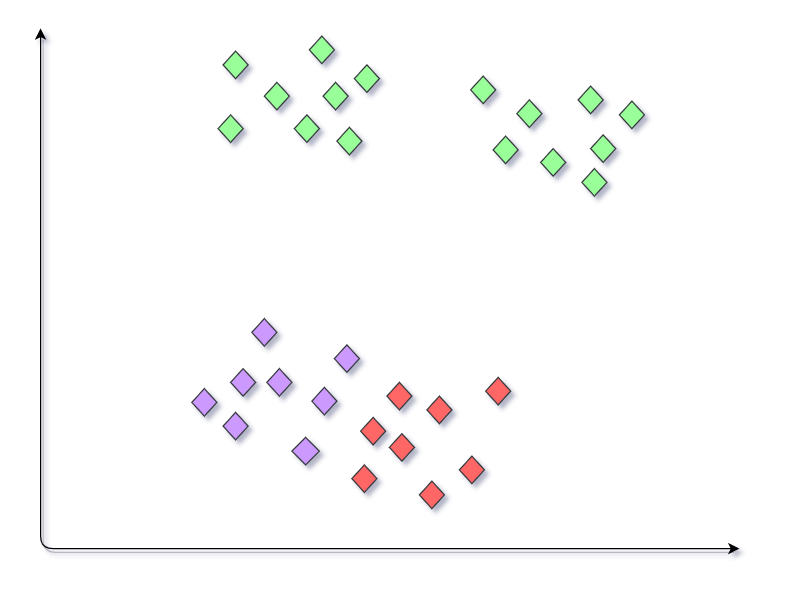
\includegraphics[width=.9\linewidth]{./Chapitre2/figures/kmeans1.png}
  \end{subfigure}
  \begin{subfigure}{.49\textwidth}
    \centering
    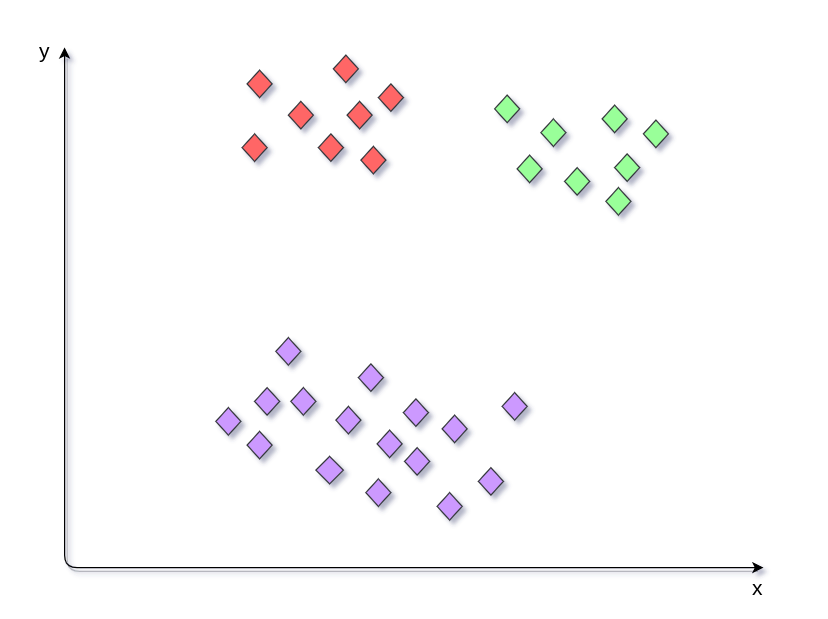
\includegraphics[width=.9\linewidth]{./Chapitre2/figures/kmeans2.png}
  \end{subfigure}
  \caption{Deux classifications en 3 classes utilisant l'algorithme k-moyennes avec deux initialisations de centroides différentes. Ici les données sont des points de coordonnées $(x,y)$. Illustrations issues de shorturl.at/htMN6 .}
  \label{fig:kmeans}
\end{figure}

%
% Les réseaux de neurones sont eux aussi impactés par l'initialisation. En plus de dégrader les performances de la classification, une mauvaise initialisation peut allonger le temps d'apprentissage voir même empêcher la convergence des systèmes. Il est donc important de considérer l’initialisation des systèmes comme un paramètre majeur de l'apprentissage automatique.
%
% %L’initialisation n'est pas le seul facteur à considérer lors d'un apprentissage automatique.
%
% \subsection{La régularisation}
% L’initialisation a son importance dans la performance d'un réseau de neurones, comme nous l'avons vu précédemment. Mais une bonne initialisation n'est pas suffisante pour garantir un système performant. Un des problèmes courants de l'apprentissage automatique est le sur-apprentissage. Ce problème peut être réglé par des méthodes dites de régularisation. Le sur-apprentissage et la régularisation sont définis dans cette section.
%
% \subsubsection{Le problème du sur-apprentissage}
% Le sur-apprentissage, overfitting en anglais, est aussi appelé sur-ajustement. Il s'agit d'un phénomène naturel présent dans l'apprentissage lors duquel le système apprend à émettre les sorties exactes demandées pour les données d'apprentissage. Cela peut être rapproché de l'apprentissage par cœur chez les humains. En effet, ce phénomène intervient quand le nombre de paramètres d'un réseau est trop important, et quand le nombre de données d'apprentissage est trop faible. Alors la minimisation de l'erreur de prédiction, définie par la fonction de coût, conduira un système à parfaitement s'aligner aux données d’entraînement. On dit que ces systèmes sont très spécialisés et qu'ils ne sont pas capables de généraliser. En effet, lorsque nous lui présentons de nouvelles données, il ne pourra pas les modéliser et donnera des sorties proches de celles des données d’entraînement et non proches de celles des données réelles.
%
% Pour rappel, on distingue les données d'apprentissage (train en anglais), des données de développement (dev en anglais) et de test. Seules les données d'apprentissage sont données au système pendant la phase d'apprentissage. On utilise ensuite les données de développement pour mesurer les performances du système et on ajuste les hyper-paramètres afin d'obtenir un système performant sur ces données qui ne sont pas utilisées lors de l'apprentissage. Les données de test permettent de donner un score final au système, permettant de le comparer à d'autres systèmes testés sur ces mêmes données de test.
%
% Le phénomène de sur-apprentissage est facilement identifiable : le score de la fonction de coût est très bon sur les données d’entraînement et très mauvais sur les données de développement et de test. Il suffit donc de vérifier l'écart entre les scores associés aux données d’entraînement et aux données de développement.  Si cet écart est trop prononcé et que le score sur les données d’entraînement est très bon, on peut en conclure que l'on se situe dans une configuration de sur-apprentissage.
% \begin{figure}[ht]
  \centering
  \begin{subfigure}{.49\textwidth}
    \centering
    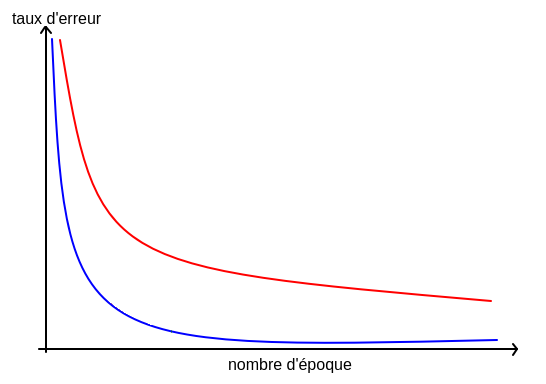
\includegraphics[width=.9\linewidth]{./Chapitre2/figures/surapprentissage2.png}
  \end{subfigure}
  \begin{subfigure}{.49\textwidth}
    \centering
    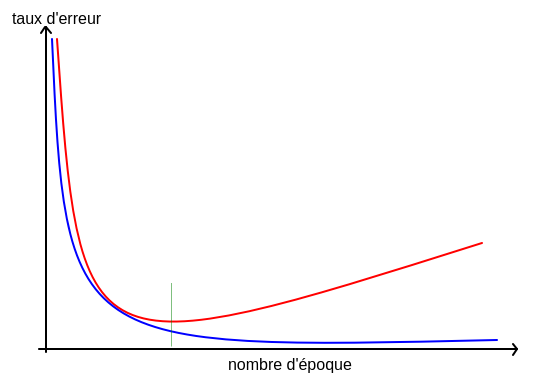
\includegraphics[width=.9\linewidth]{./Chapitre2/figures/surapprentissage1.png}
  \end{subfigure}
  \caption{Deux évolutions de scores sur les données d'entrainement en bleu et de développement en rouge. La figure de droite correspond à une situation de sur-apprentissage. Cette situation est observable à partir de l'époque correspondant à la ligne verte tracée.}
  \label{fig:surapprentissage}
\end{figure}

%
% On peut voir sur la figure~\ref{fig:surapprentissage} l'évolution des scores constatés sur un ensemble d'apprentissage et un ensemble de développement. Dans la partie gauche, on constate une évolution normale des scores d'apprentissage sur l’entraînement (en bleu) et sur le développement (en rouge). Dans la partie droite, on remarque le sur-apprentissage qui commence à la période où les deux courbes évoluent en sens contraires. Le modèle apprend par cœur les données d'apprentissage et n'arrive plus à généraliser aux données de développement.
%
% Plusieurs méthodes permettent de palier à ce phénomène. On a tout d'abord les méthodes passives, qui vont détecter les modèles en sur-apprentissage pour les supprimer. C'est ce que l'on met en place en utilisant un ensemble de développement ou de validation. On peut également diminuer le nombre de paramètres, en modifiant l'architecture neuronal ou augmenter le nombre de données d’entraînement.
%
% Il y a également les méthodes actives, qui sont également appelées méthodes de régularisation servant à contrôler la valeur des poids des neurones lors de l'apprentissage. Bartlett~\cite{Bartlett1997} a démontré que la valeur des poids est plus importante que le nombre de poids et donc de neurones pour éviter le sur-apprentissage. Nous allons considérer les régularisations les plus communes dans les prochains paragraphes.
%
% \subsubsection{Régularisation L1 et L2}
%
% La régularisation L1, ou Lasso Regression (Least Absolute Shrinkage and Selection Operator en anglais) a été introduite par Tibshirani~\cite{Tibshirani1996}. La régularisation L2 (Ridge Regression en anglais) quant à elle a été introduite par Hoerl et Kennard~\cite{Hoerl1970}. Ces deux régularisations mettent en place une pénalité $p\geq 0$ qui est ajoutée à la fonction de coût. Elles diffèrent cependant sur la norme (L1 ou L2)%(L1 décrite par l'équation~\ref{eq:L1} ou L2 décrite par l'équation~\ref{eq:L2})
% utilisée pour calculer cette pénalité. Utilisées pour pénaliser les poids les plus élevés, elles vont permettre la désactivation de certains neurones. %$w_i$ correspond au poids du neurone $i$ et $\lambda$ à un coefficient fixé par l'humain.
%
% % \begin{equation}
% %   p = \lambda\sum_{i=1}|w_i|
% %   \label{eq:L1}
% % \end{equation}
% %
% % \begin{equation}
% %   p = \lambda\sum_{i=1}w^{2}_i
% %   \label{eq:L2}
% % \end{equation}
%
% Ces deux pénalités sont assez similaires. Soit on utilise la somme de la valeur absolue des poids pour L1, soit la somme des carrées des poids pour L2. %Ces deux pénalités sont donc toujours positives.
%
% \subsubsection{Normalisation des batchs}
% Introduit par Ioffe et al.~\cite{Ioffe2015}, cette régularisation, appelée Batch Normalization en anglais, cherche à réduire les variations des données d'entrées de chacune des couches. Toutes les informations connues dans un réseau neuronal sont inscrites dans un espace. L'objectif de l'apprentissage est de retrouver la meilleure représentation de ces informations de sorte que toutes les données d'une même classe soit dans le même espace. On appelle l'éloignement entre les informations, le décalage des co-variables (covariate shift en anglais). Cet éloignement peut être observé entre toutes les représentations, qu'elles soient considérées de la même classe ou non. Cependant cet écart doit être réduit pour les données ayant la même étiquette de sortie.
%
% Une des façons de s'affranchir de ce problème est d'utiliser des lots, comme nous l'avons vu précédemment. Mais l'utilisation de lots ne va pas réduire la distance entre les représentations apprises par le système. Cette régularisation cible donc les représentations intermédiaires des données, à l'intérieur des couches cachées.
%
% %L'objectif de cette méthode est de réduire le décalage des co-variables dans les couches cachées.
% Pour ce faire, on applique une normalisation à chaque entrée de neurones, quelque soit sa position dans les couches de façon individuelle. La normalisation est calculée avec la moyenne $\mu$ et la variance $\sigma$ d’un lot ($B$), avec les équations~\ref{eq:mu} et~\ref{eq:rho} dans lesquelles $n$ représente le nombre d'éléments du lot et $z^i$ la valeur d'activation du neurone normalisé lors de l'itération $i$.
% \begin{equation}
%   \mu_B = \frac{1}{n} \sum^n_{i=1}{z^i}
%   \label{eq:mu}
% \end{equation}
% \begin{equation}
%   \sigma^2_B = \frac{1}{n} \sum^n_{i=1}{(z^i-\mu_B)^2}
%   \label{eq:rho}
% \end{equation}
%
% Avec la moyenne et la variance, on peut alors appliquer la normalisation selon l'équation~\ref{eq:normBatch}. $\epsilon$ est un coefficient faible ajouté pour éviter les divisions par zéro. Enfin la valeur d'échelle $\gamma$ et la valeur de décalage $\beta$ sont des paramètres qui sont appris pendant l'apprentissage.
% \begin{equation}
%   z'^i = \gamma \left ( \frac{z^i-\mu_B}{\sqrt{\sigma^2_B + \epsilon}} \right ) + \beta
%   \label{eq:normBatch}
% \end{equation}
%
% Cette normalisation permet d'éviter le sur-apprentissage. Elle permet également d'accélérer la mise en place de représentations internes cohérentes et donc de diminuer le temps d'apprentissage.
%
% \subsubsection{Arrêt prématuré de l'apprentissage}
% Une autre méthode de régularisation largement utilisée consiste à arrêter l'apprentissage de façon précoce en fonction de la variation de l'erreur calculée à chaque époque. En effet, si la variation de l'erreur est trop faible, il est très probable que l'on ait atteint un minimum local acceptable. Continuer l'apprentissage ne serait alors qu'une source possible de sur-ajustement. Cette méthode, appelée early stopping~\cite{Prechelt1998}, peut être appliquée sur l'erreur calculée sur les données d'apprentissage ou sur l'erreur calculée sur les données de développement.
%
% Bien que simpliste au premier abord, cette méthode est souvent utilisée car elle est une normalisation très efficace~\cite{Finnoff1993} qui assure que le système ne sur-ajuste pas. De plus, elle permet de réduire le temps d'apprentissage, puisqu'elle diminue la plupart du temps, le nombre d'époques effectuées.
%
% \subsubsection{L'utilisation du dropout}
% Le dropout, introduit par Srivastava et al.~\cite{Srivastava2014} est une normalisation très utilisée de nos jours. Elle consiste en la désactivation temporaire et aléatoire de neurones à une époque donnée. Ainsi, le réseau a toujours des poids à apprendre et cela évite de tomber dans un phénomène de sur-apprentissage. Comme le réseau est privé de certains de ces neurones, il doit apprendre à compenser cette perte, ce qui rend les représentations internes plus robustes et améliore la généralisation du modèle.
%
% Ainsi, en fonction d'une probabilité de désactivation des neurones, souvent fixée à $0.5$, le réseau aura plus ou moins de neurones désactivés et devra palier à ce manque de représentation.
%
% Toutes ces méthodes permettent de garantir un fonctionnement correct voir optimal d'un système neuronal, et cela quelque soit l'architecture des réseaux de neurones employée.

\section{Les architectures des réseaux dans le traitement du signal}

Dans le cadre de cette thèse, nous travaillons sur les informations contenues dans le signal. %Ces informations étant par nature plutot massive, il est interessant d'utiliser des réseaux de neurones pour les traiter.
Cependant l'utilisation du perceptron multi-couche (MLP) n'est pas la plus performante des approches pour représenter les données de type parole. Il existe d'autres architectures de couches neuronales bien plus pertinentes avec ces données. En effet, le principal inconvénient du MLP, c'est que les segments de parole sont considérés un à un, il est donc difficile de gérer les relations temporelles par exemple : on ne prend pas en compte le contexte. Le passé et le futur n'influencent pas directement les systèmes d'apprentissage. Une entrée est donc considérée seule et sans contexte.

Or nous savons que la parole est caractérisée par l'entièreté de sa séquence. Si nous faisons un parallèle avec un texte, une lettre seule ne veut rien dire. Accompagnée d'autres lettres, elles forment un mot. Ces mots sont eux-mêmes agencés avec d'autres mots pour donner un sens à une phrase.

Comme le contenu d'un segment de parole à un instant $t$ dépend des instants précédents, il est nécessaire d'utiliser des réseaux permettant de prendre en compte les segments précédents voir les segments suivants. Dans cette section, nous allons décrire les architectures neuronales permettant de conserver l'historique des états précédents, qui sont par conséquent utilisées dans le traitement de la parole.

\subsection{Réseaux neuronaux convolutifs}
Les réseaux neuronaux convolutifs (Convolutional Neural Network en anglais), abrégés CNN~\cite{LeCun1989} sont prépondérants dans l'analyse d'image. En effet les CNNs traitent des données représentées en $n$ dimensions comme des images (disposition des pixel en 2D), permettant des résultats probants sur des tâches de reconnaissance d'écriture manuscrite de chiffres et de nombres~\cite{LeCun1998}, de reconnaissance d'objets au sein d'une image~\cite{Traore2018}, ou de reconnaissance de visages~\cite{Liu2016}. Ils sont également utilisés en parole, lorsque l'on considère le signal comme un spectrogramme par exemple~\cite{Abdel2014}. Récemment, cette architecture a été utilisée pour répondre à des tâches concernant la reconnaissance d'émotions, aussi bien à partir d'images de visage~\cite{Pitaloka2017,Mehendale2020} qu'à partir de signaux de parole~\cite{Zhang2016}.

\begin{figure}[h]
  \centering
  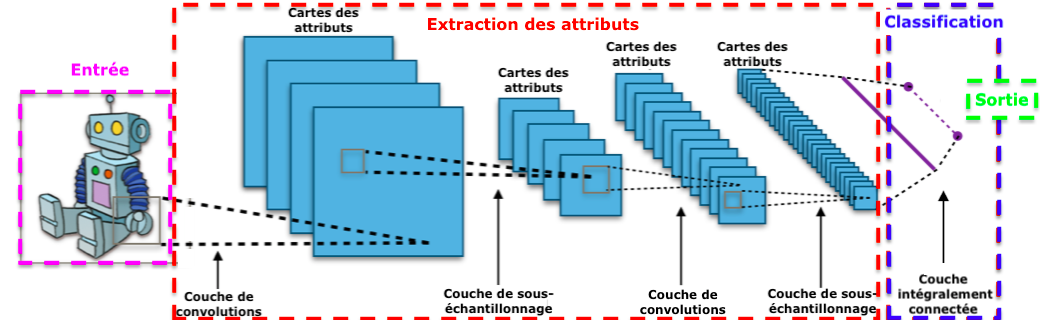
\includegraphics[width=14cm]{./Chapitre3/figures/cnn.png}
  \caption{Représentation schématique du traitement d'une image par un réseau de type convolutionnel. Image provenant de Wikipedia.}
  \label{fig:cnn}
\end{figure}


Comme nous l'avons vu précédemment, ils sont pertinents dans le traitement des images, puisque ces dernières se représentent sous la forme d'une addition de tableaux de 2D (trois pour des images RGB, quatre si on considère la transparence de l'image, un seul pour une image en noir et blanc).
Le CNN va découper les tableaux en fenêtres. Il va ensuite chercher ces fenêtres dans les nouvelles données qui lui sont présentées, il va donc opérer un filtrage. Ce filtrage est effectué pour chaque fragment de la donnée.
% Comme son nom l'indique, ce réseau effectue des produits de convolutions en fonction de la configuration de son champ récepteur. Il se décompose en trois opérations : la convolution, le pooling puis l'activation de type ReLu.
% Si nous revenons dans le détail, ils ont été conçus pour des données présentées sous forme de tableaux de N dimensions.

On peut décrire le fonctionnement d'un réseau convolutif par une succession d'étapes, présentée dans la figure~\ref{fig:cnn} :

\begin{itemize}
  \item l'étape de convolution consiste à faire glisser le filtre sur l'ensemble du tableau et à calculer le produit de la convolution entre chaque fenêtre et le filtre. Cette étape est répétée pour couvrir tout le tableau et utilise un filtre de même taille pour chaque fenêtre.
  \item l'étape de sous-échantillonnage (pooling en anglais) va permettre de réduire la taille totale du tableau tout en conservant les informations pertinentes pour le système. Différentes méthodes de sous-échantillonnage existent mais les plus usitées sont les fonctions mathématiques de type minimum, maximum ou moyenne du tableau. Cette étape est importante, puisqu'elle permet de garantir une réduction du nombre de paramètres, qui peut augmenter très rapidement avec les couches de convolution.
  \item optionnellement, on peut ajouter des couches denses.%des étapes de correction. Ces couches ont pour rôle de faciliter la prise de décision au sein du réseau, en activant ou désactivant certaines connexions entre les différents neurones. Elles se présentent sous la forme de fonctions mathématiques qui vont être appliquées en sortie d'une couche. Principalement on retrouve la fonction ReLU, la tangente hyperbolique et la fonction sigmoïde.
\end{itemize}

%Il y a donc deux hyper-paramètres spécifiques à considérer lors de la construction d'un réseau convolutif : le nombre de caractéristiques, qui va déterminer la taille du filtre et le pas qui va contrôler les chevauchements.

Le CNN a pour avantage de couvrir la plupart du temps l'intégralité des données pour retrouver une caractéristique. Ainsi, même si cette dernière n'est pas présente au même endroit dans les nouvelles données, elle sera retrouvée. De plus, grâce à l'étape de pooling, le nombre de paramètres se voit fortement réduit, ce qui permet d'obtenir de bonnes performances pour un temps et un usage mémoire réduit.

Cependant le CNN %a besoin de beaucoup de données pour ne pas être sur-appris et suivant ses hyper-paramètres, il peut ne jamais converger. De plus, ils ont
a besoin de séquences d'entrée de taille fixe, ce qui n'est pas très adapté quand on pense à de la parole.

\subsection{Réseaux Neuronaux Récurrents}
\begin{figure}[h]
  \centering
  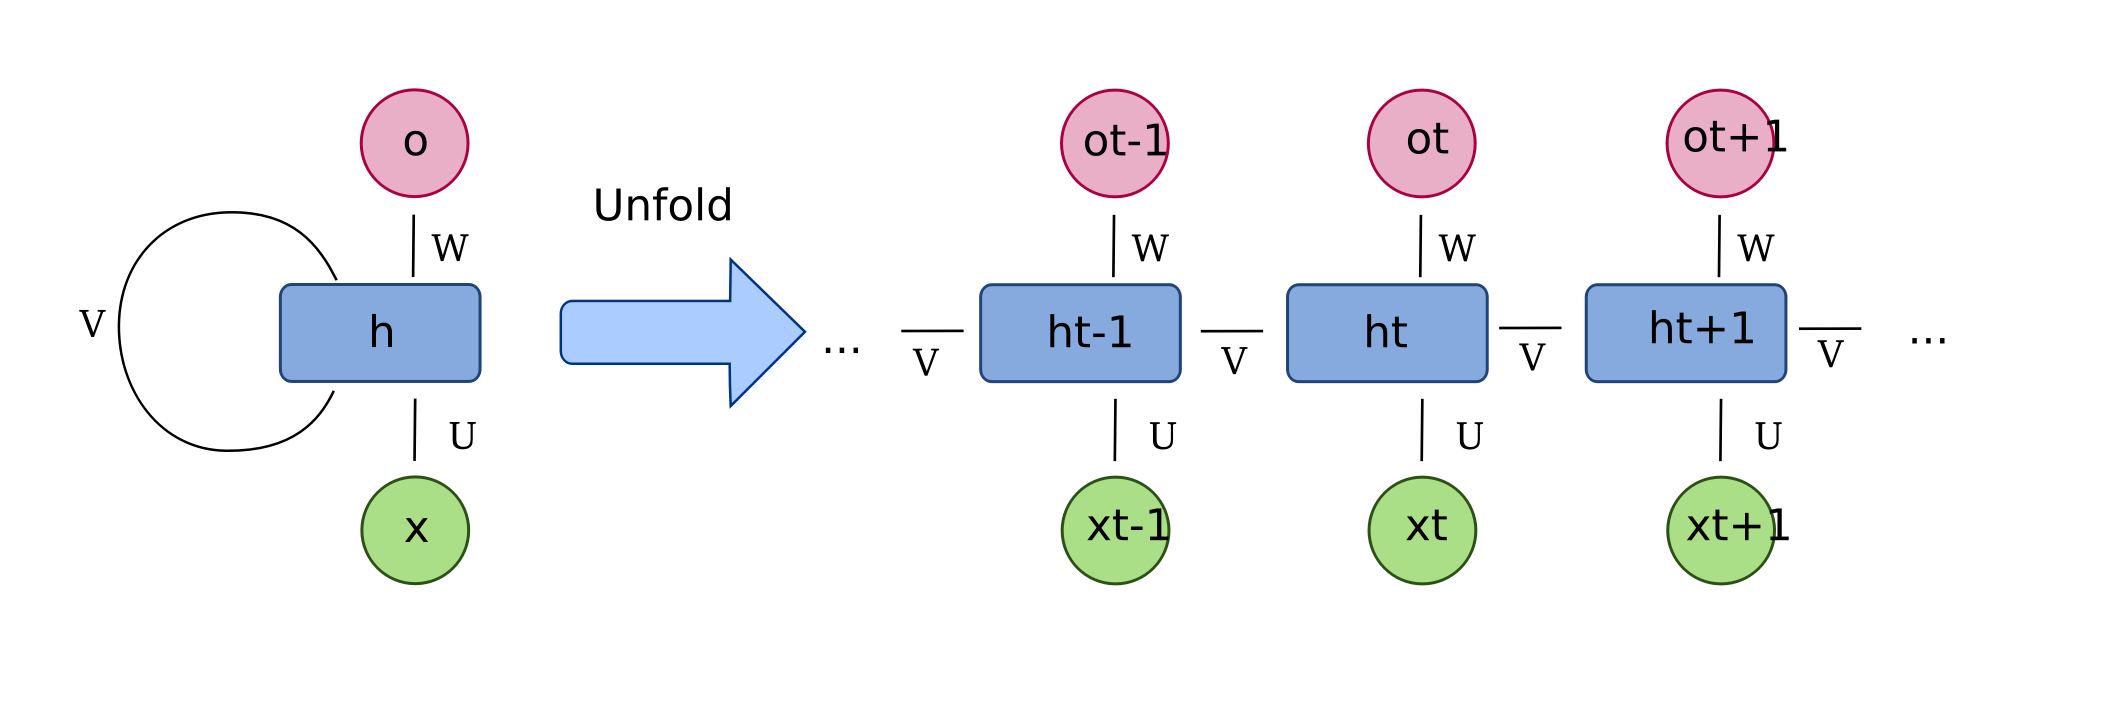
\includegraphics[width=14cm]{./Chapitre3/figures/rnn.png}
  \caption{Représentation schématique d'un réseau neuronal récurrent. La partie gauche correspond à une récurrence sur une couche entière $h$. La partie droite explicite la récurrence au niveau de la couche $h$. Image provenant de Wikipedia.}
  \label{fig:rnn}
\end{figure}


Les réseaux neuronaux récurrents (RNN)~\cite{Jordan1986} décrivent une architecture neuronale qui est très utilisée de nos jours pour résoudre de nombreuses tâches. En effet, ils permettent de modéliser des séquences (que ce soit des segments de parole, ou des vecteurs de descripteurs par exemple) dont la taille est variable, en présentant toutes les données de manière séquentielle au système. Il est donc possible de faire correspondre plusieurs entrées à plusieurs sorties (appelé \textit{many-to-many}) ainsi que plusieurs entrées à une seule sortie (appelé \textit{many-to-one}). %contrairement aux perceptrons multi-couches, permettant uniquement de faire correspondre une entrée à une sortie (appelé \textit{one-to-one}).

Ils permettent également de prendre en compte l'aspect chronologique, ou antéchronologique si nécessaire, de la séquence et met en avant les dépendances temporelles dans les séquences.
Pour modéliser cet aspect mémoriel, une deuxième entrée est ajoutée au neurone, correspondant à la sortie précédente dans la séquence, comme explicité dans le schéma~\ref{fig:rnn}. Cette boucle va donc permettre de conserver des informations entre les différentes itérations du système.

Même si en théorie leur mémoire devrait pouvoir contenir tous les éléments de la séquence visualisée, ce n'est pas le cas dans les faits. Bengio et al.~\cite{Bengio1994} ont montré que ces systèmes ont beaucoup de mal à modéliser des dépendances éloignées. On pourra difficilement modéliser une dépendance entre un début de conversation et sa fin si la séquence est trop longue par exemple.

C'est pour pallier ce problème qu'un autre type de réseau récurrent a été développé.

\subsection{Réseaux long-short term memory}
\begin{figure}[h]
  \centering
  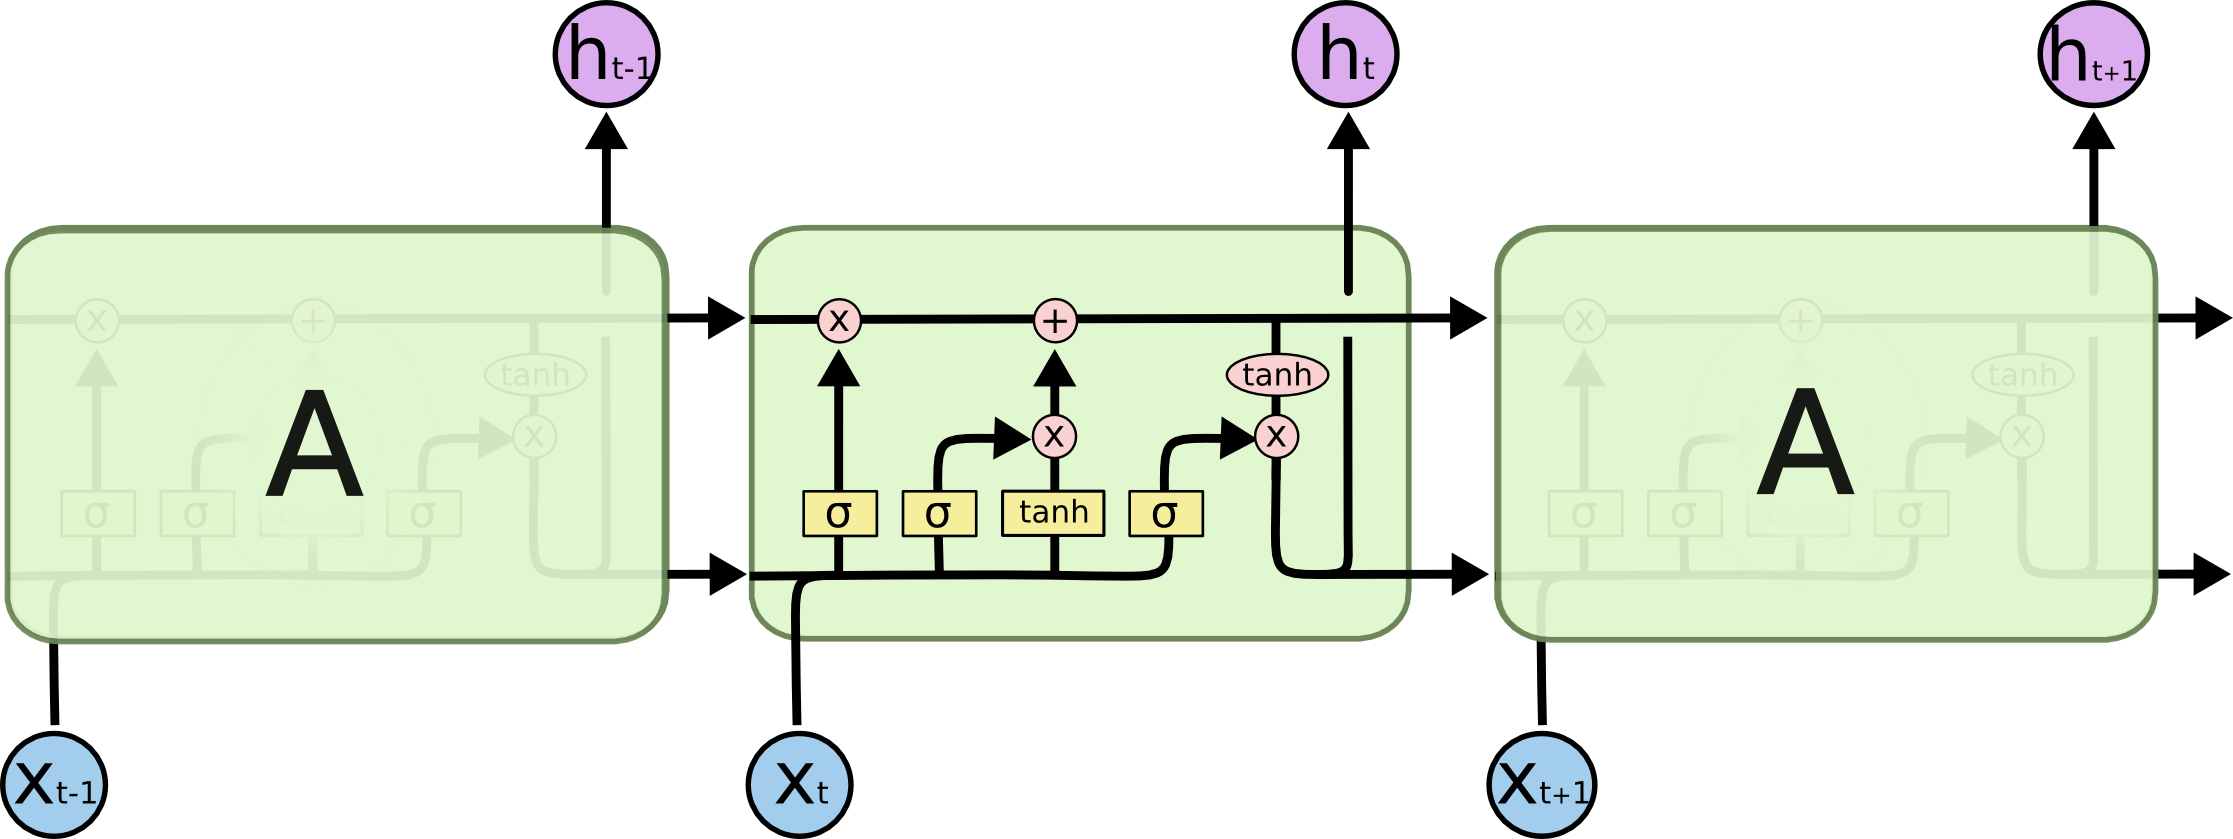
\includegraphics[width=14cm]{./Chapitre3/figures/lstm.png}
  \caption{Représentation schématique d'un réseau récurrent à mémoire court et long terme (LSTM). On observe qu'il y a deux entrées à l'unité neuronale : l'état de la cellule (cell state) en haut et la sortie classique d'un neurone en bas. Image provenant de http://colah.github.io/posts/2015-08-Understanding-LSTMs/ .}
  \label{fig:lstm}
\end{figure}


Les réseaux \textit{long-short term memory} (LSTM)~\cite{Hochreiter1997} ont été crés pour répondre à la perte de la mémoire longue des RNN. Présentés dans la figure~\ref{fig:lstm}, ils sont spécialisés dans la modélisation de dépendances éloignées dans une séquence, en fonctionnant avec une mémoire interne à chaque neurone (\textit{cell state}) qui permet de modéliser des dépendances à des instants éloignés dans la séquence.

Lorsque la sortie de l'unité neuronale précédente $h_{t-1}$ arrive dans l'unité courante $t$, elle va passer par trois portes, utilisant des sigmoïdes et des tangentes hyperboliques. La première porte, \textit{la porte de l'oubli}, est en charge de la suppression d'informations non pertinentes stockées dans la mémoire interne (cell-state en anglais). La deuxième porte, la porte d'entrée, va décider des nouvelles informations à ajouter dans la mémoire interne. Elle est alors mise à jour avec les informations ajoutées et retirées. La dernière porte, la porte de sortie, est en charge de la sortie effective. Elle est calculée en fonction de la mémoire interne mais aussi de l'état courant en utilisant une tangente hyperbolique pour forcer les valeurs entre -1 et 1 puis une dernière sigmoïde afin de ne transmettre que les informations activées.

Cette architecture existe également de façon bidirectionnelle : la séquence est lue dans l'ordre chronologique  et antéchronologique. Pour avoir ces deux directions, on multiplie le nombre de couches du système par deux : une prenant les informations dans l'ordre et une autre prenant les informations dans l'ordre inverse. Enfin les sorties des deux couches sont concaténées pour donner la sortie finale de chaque élément. Cela permet de mettre en évidence les dépendances passées et futures.

Cette architecture est pertinente pour toutes les données qui ont besoin de contexte. C'est pour cela qu'elle est très utilisée dans le domaine du traitement de la parole notamment. Cependant, le temps d'apprentissage est long puisqu'il y a beaucoup de paramètres à apprendre et qu'il est difficile de paralléliser les calculs au vu de son caractère séquentiel. De plus, dans le cas du LSTM bidirectionnel, nous avons besoin de la séquence en entier pour avoir une prédiction, ce qui n'est pas forcément compatible avec du temps réel.

\subsection{Encodeur Décodeur}
\begin{figure}[h]
  \centering
  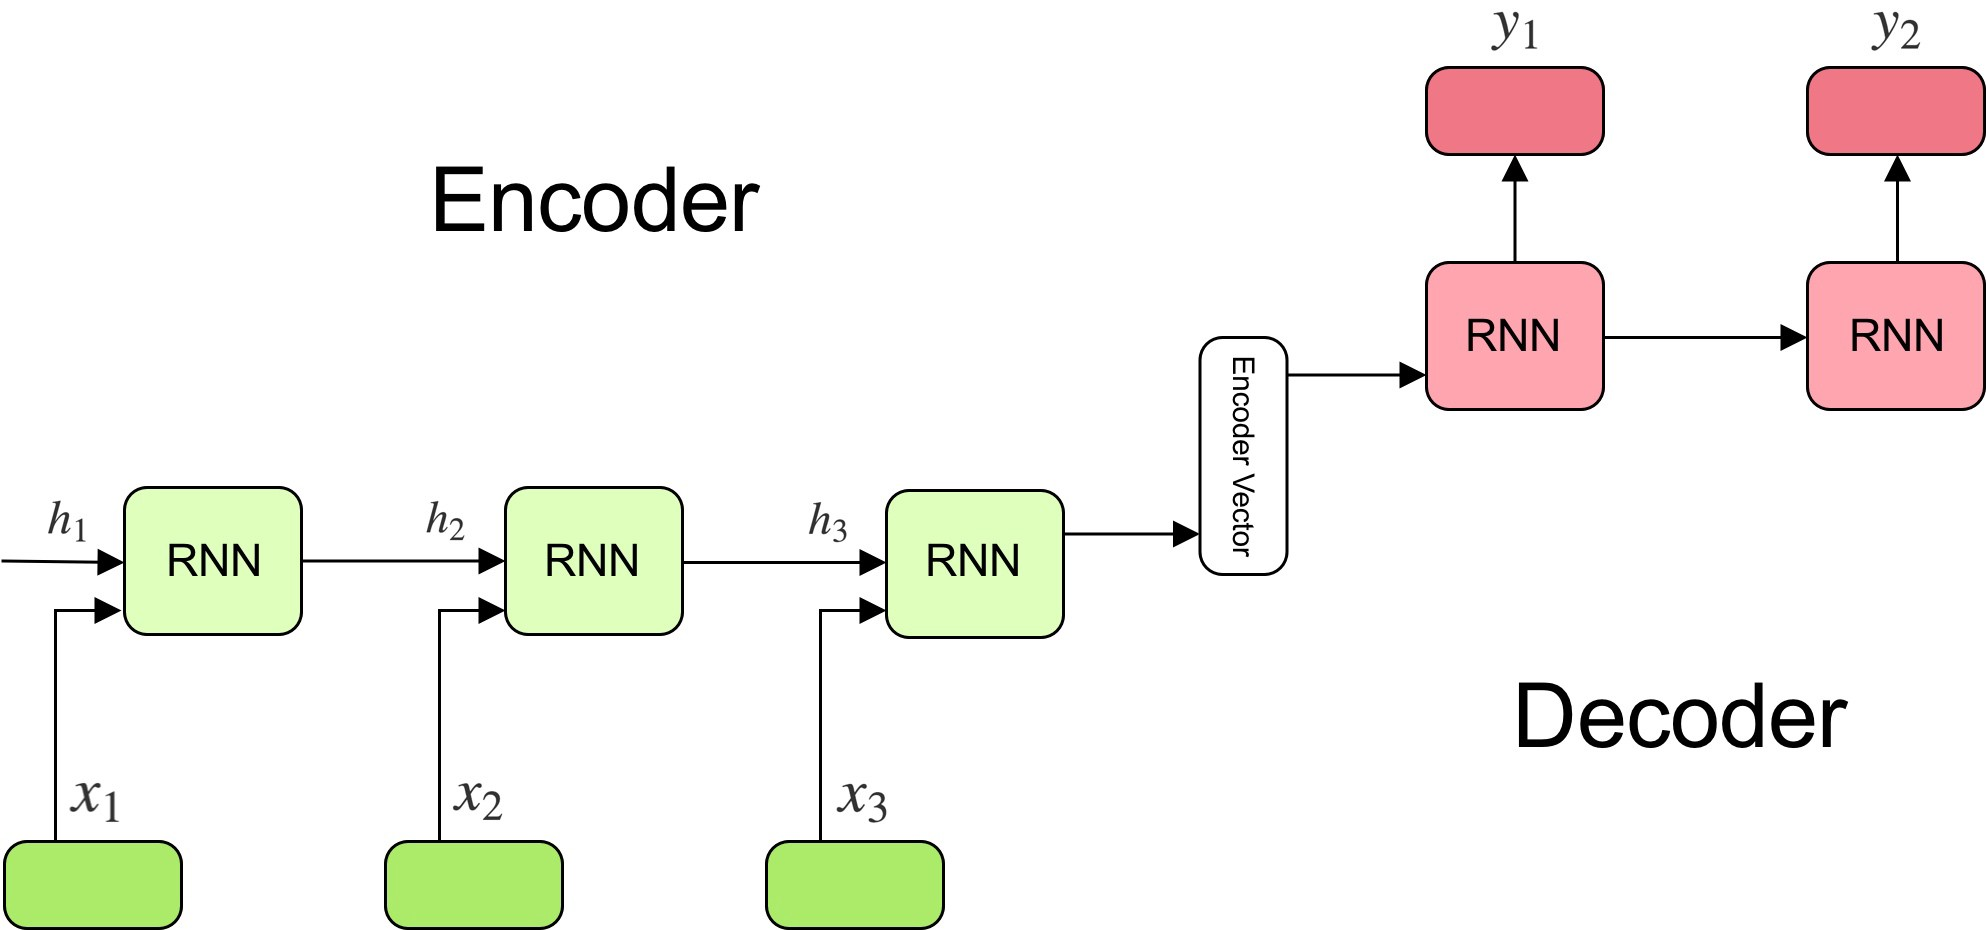
\includegraphics[width=14cm]{./Chapitre3/figures/encoder.jpeg}
  \caption{Représentation schématique d'un système encodeur décodeur. $x_i$ correspondent aux entrées, $y_i$ aux sorties. Image provenant de shorturl.at/dmsCS}
  \label{fig:encoder}
\end{figure}


Conçu dans les années 2010, l'encodeur décodeur (Encoder-Decoder en anglais)~\cite{Cho2014} se compose, comme son nom l'indique, de deux parties distinctes. Ces deux parties sont utilisées conjointement pour prédire une ou plusieurs sorties $y_i$ comme illustré par la figure~\ref{fig:encoder}.

Un encodeur correspond à un réseau de neurones récurrent qui transforme une séquence d'entrée $X$ en une représentation vectorielle de taille fixe $X'$. Une fois cette première transformation effectuée, le décodeur, correspondant lui aussi à un RNN, transforme cette représentation intermédiaire $X'$ en une séquence de sortie $Y$. Cette transformation finale est calculée en fonction de la distribution de probabilité de toutes les sorties possibles $P(Y|X')$.

Il existe un cas particulier de cette architecture, que l'on nomme les auto-encodeurs. Ce sont des réseaux qui possèdent exactement le même nombre de neurones sur leur couche d'entrée et leur couche de sortie. L'objectif de ces réseaux est d'avoir une sortie la plus proche possible de l'entrée. Ils permettent notamment de débruiter des données d'entrée ou de créer des nouvelles données dans le cadre de l'augmentation de données.

L'encodeur décodeur a notamment prouvé sa pertinence dans des tâches de reconnaissance de la parole~\cite{Chiu2018}, dans des tâches de NLP~\cite{Hu2019} ou dans des tâches de traduction~\cite{Cho2014} par exemple.

Néanmoins cette architecture peut avoir des difficultés à modéliser les dépendances qui sont trop éloignées dans la séquence courante. Un moyen de contourner ce problème est d'utiliser des mécanismes d'attention~\cite{Bahdanau2016}. En effet, le modèle peut concentrer son attention sur les parties qu'il juge pertinentes, où qu'elles soient dans la séquence d'entrée.

\subsubsection{Mécanismes d’attention}

Les mécanismes d'attention ont d'abord été utilisés dans le cadre de la traduction automatique~\cite{Luong2015}, avant d'être rapidement étendus à toutes tâches utilisant des séquences.

Les mécanismes d'attention apportent plusieurs concepts aux encodeurs décodeurs. Tout d'abord, ils étendent les informations contenues dans les états cachés : au lieu de ne fournir que le dernier état caché de l'encodeur, l'ensemble des états cachées pour chacune des entrées précédentes est fourni.

De plus, le vecteur de contexte est pondéré en fonction de la pertinence des informations qu'il contient pour chacun des états émis par l'encodeur. Cette pondération est produite par un score d'attention, compris entre 0 et 1. De ce fait, le vecteur de contexte est composé de la somme des états cachés calculés par l'encodeur pondérés par les scores d'attention.

Enfin le vecteur de contexte devient dynamique : il est recalculé afin de mieux cibler les informations pertinentes dans la séquence d'entrée.

\subsection{Transformers}

Les Transformers sont issus des travaux de Vaswani et al.~\cite{Vaswani2017}. Il s’agit d’un modèle qui utilise une architecture encodeur décodeur mais qui met en place des mécanismes d’attention différents. Elle correspond à un empilement de plusieurs encodeurs et décodeurs. Le nombre d’encodeurs et de décodeurs est identique au départ. Maintenant ce n'est plus forcément le cas.

Dans le cas des Transformers, un encodeur est composé d’un bloc d’auto-attention (\textit{self-attention}), suivie d’une couche linéaire. Le décodeur est lui aussi complété par une couche d’attention. De plus, les Transformers ont introduit les mécanismes d’attention à plusieurs têtes (\textit{multi-head attention}).

Ils sont très performants mais également très coûteux à l'apprentissage. En effet, ils sont composés de beaucoup de paramètres du fait de l'architecture, ce qui se traduit par un long temps de convergence, et un besoin de très grandes quantités de données. Cependant ces inconvénients peuvent être en partie gommé par un apprentissage parallélisable. Ils ont notamment contribué à la création de modèles pré-appris.


\section{Modèles pré-entraînés}

La méthode de transfert d'apprentissage (\textit{transfer learning} en anglais)~\cite{Goodfellow2016} dans le paradigme de l'apprentissage profond est une méthode d'apprentissage automatique dans laquelle un réseau de neurones entraîné pour une tâche ou un domaine est réutilisé partiellement ou entièrement comme point de départ pour entraîner ou affiner un réseau de neurones sur une autre tâche ou un autre domaine, comme nous l'avons vu précédemment. Cette méthode permet notamment de limiter l'impact du manque de données sur des réseaux de neurones.
Elle est largement utilisée dans l'analyse d'émotions, où de grandes bases de données sont utilisées pour pré-apprendre les poids des réseaux, conduisant à de meilleures capacités de généralisation compte tenu des données d’entraînement limitées~\cite{Dong2018}.

Parmi les techniques de transfert d'apprentissage, l'apprentissage auto-supervisé des représentations de la parole ou du langage (\textit{self-supervised learning of speech or language representations}) a émergé ces dernières années avec l'introduction du modèle BERT~\cite{Devlin2019}.

\subsection{Représentation linguistique}
Parmi les représentations linguistiques, les plongements de mots (\textit{word embedding}) sont l'une des représentations continues de données textuelles les plus populaires. Ces plongements sont des représentations vectorielles d'un mot particulier. Pour les calculer, on peut utiliser Word2vec~\cite{word2vec} qui est un des modèles les plus utilisés pour apprendre des plongements de mots dans les tâches d'analyse des sentiments telles que la polarité ou la classification des états émotionnels~\cite{Rodrigo2020,Dong2018}. Les plongements de mots obtenus avec Word2vec sont statiques : un mot a toujours la même représentation vectorielle, quel que soit le sens du mot et le contexte de son apparition. Ce qui est problématique pour les mots polysémiques par exemple, qui sont fréquents en français~\cite{Pustejovsky1996}.

\subsubsection{BERT}
D'autres modèles sont sortis ces dernières années, comme BERT~\cite{Devlin2019} (entraîné sur des données anglaises puis sur des données multilingues) ou Ernie~\cite{Zhang2019Ernie} (entraînés sur des données chinoises ou des données anglaises) qui est dépendant du langage et du contexte. Ces modèles ont besoin de beaucoup de données pour être entraînés : ils utilisent notamment le corpus de Wikipédia totalisant plus de 2 500 millions de mots et le Book Corpus~\cite{Zhu2015} totalisant plus de 800 millions de mots.

BERT est l’acronyme de \textit{Bidirectional Encoder Representations from Transformers}. Il existe deux modèles BERT disponibles, le \textit{BASE} et le \textit{LARGE}. Comme leur nom l'indique, ils sont composés d'un nombre plus ou moins important de blocs d'encodeurs de type Transformers pour un total de 110 millions de paramètres pour le modèle BASE et 340 millions de paramètres pour le modèle LARGE.
% , qui correspondent à des Transformers :
% \begin{itemize}
%   \item \textit{BASE} : 12 blocs d'encodeurs de tyTransformers, 768 couches cachées, 12 têtes d'attention pour un total de 110 millions de paramètres.
%   \item \textit{LARGE} : 24 Transformers, 1024 couches cachées, 16 têtes d'attention pour un total de 340 millions de paramètres.
% \end{itemize}

Ce modèle est pré-appris sur deux tâches distinctes : la tâche \textit{Masked LM} où certains mots sont masqués dans les données et le système apprend à les prédire, ainsi que la tâche \textit{Next Sentence Prediction} où le système apprend à prédire la phrase suivante. Une fois ce pré-apprentissage effectué, le modèle BERT est appris. Ces deux étapes sont illustrées par la figure~\ref{fig:BERT}. Dans l'article de Devlin et al.~\cite{Devlin2019}, 11 tâches de NLP ont été effectuées pour montrer les performances du modèle BERT ainsi appris.   %\textit{fine-tuning} réalisé sur 11 tâches de NLP différentes.

\begin{figure}[h]
  \centering
  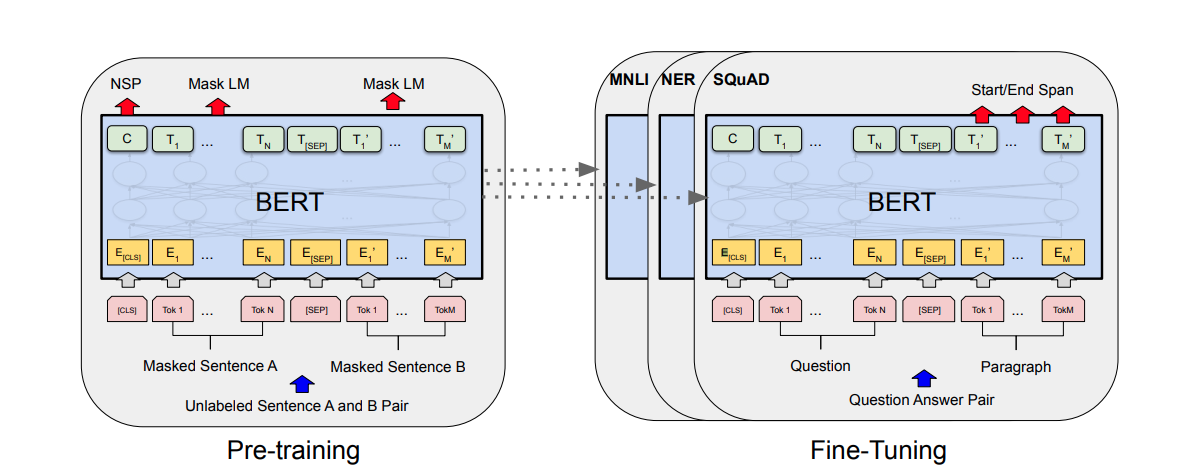
\includegraphics[width=16.5cm]{./Chapitre2/figures/bert.png}
  \caption{Représentation graphique des deux étapes permettant d'obtenir le modèle BERT. Issue des travaux de Devlin et al.~\cite{Devlin2019}}
  \label{fig:BERT}
\end{figure}


Ce modèle a montré son efficacité sur certaines tâches, par exemple %pour la vision par ordinateur~\cite{Nanni2017} et
les tâches de traitement du langage naturel (NLP) telles que la
classification de phrases, la similarité de texte, ou le classement par pertinence~\cite{Liu2019,Young2018,Yang2019}. De même cette approche montre de très bons résultats dans les domaines de l'ASR~\cite{Kahn2020,Liu2020} ou de traduction depuis la parole~\cite{Nguyen2020}.

\subsubsection{CamemBERT}
Si nous nous replaçons dans notre contexte, nous travaillons avec des données françaises. Nous nous sommes donc intéressés aux dérivées de BERT adapté pour la langue française. CamemBERT~\cite{Martin2020} et FlauBERT~\cite{Le2020} sont deux modèles appris sur des données françaises. Ces deux modèles sont accessibles \footnote{https://camembert-model.fr/}~\footnote{https://github.com/getalp/Flaubert}, permettant de mettre en place des représentations linguistiques adaptées à la langue française.

CamemBERT est appris en utilisant le système RoBERTa~\cite{Liu2019Roberta}, un système BERT amélioré avec moins d'étapes d'apprentissage mais de plus gros lot d'apprentissage et de plus gros volumes de données. Cet apprentissage est réalisé sur les données OSCAR~\cite{Ortizsuarez2019}. Ce modèle donne des résultats plutôt performants sur plusieurs tâches : l'étiquetage morphosyntaxique (\textit{part of speech} ou POS), l'analyse des dépendances sémantiques, la reconnaissance des entités nommées (NER) et l'inférence du langage naturel (NLI).
%GermanBERT~\footnote{https://deepset.ai/german-bert} models were released for German.

FlauBERT est très similaire à CamemBERT. Leurs principales différences proviennent des corpus d’entraînement et des pré-traitements qui sont différents. %De plus, ils sont complémentaires puisqu'ils répondent à des tâches NLP différentes.

Ces modèles linguistiques ont inspiré d'autres chercheurs qui ont étendu le concept à la représentation acoustique.

\subsection{Représentation acoustique}
Récemment, wav2vec~\cite{Schneider2019} et Audio AlBERT~\cite{Chi2020} ont été introduits dans le domaine de l'ASR et de l'identification du locuteur comme les premières approches pré-entraînées pour extraire des représentations acoustiques contextuelles de signaux sonores bruts.

\begin{figure}[h]
  \centering
  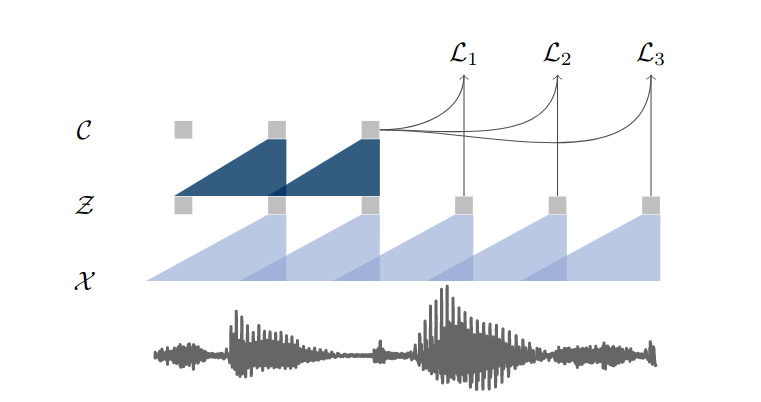
\includegraphics[width=11cm]{./Chapitre2/figures/wav2vec.png}
  \caption{Wav2vec : Schéma du pré-entraînement à partir des données audio $X$ qui sont encodées avec deux réseaux de neurones empilés. Le réseau \textit{encodeur} donne la représentation $Z$ et le réseau de \textit{contexte} donne la représentation $C$. Issu de~\cite{Schneider2019}}
  \label{fig:wav2vec}
\end{figure}


Wav2vec est entraîné sur la tâche de prédiction des futurs échantillons à partir d'une analyse de la fenêtre courante. Il est composé de deux réseaux de neurones convolutifs distincts : le réseau dit~\textit{encodeur} et celui dit~\textit{contexte} utilisés ensemble. Comme nous pouvons le voir sur la figure~\ref{fig:wav2vec}, les entrées $X$ sont d'abord replacés dans un espace latent et transformées en $Z$. Puis le réseau de \textit{contexte} va transformer ces représentations $Z$ en $C$ en combinant plusieurs pas de temps de l'encodeur précédent pour ajouter du contexte à la représentation finale.

Depuis la publication du modèle BERT, d'autres modèles pré-entraînés permettant d'obtenir une représentation acoustique ont été proposés en utilisant les blocs de Transformers et la technique de maskage, comme le modèle récent Wav2vec 2.0~\cite{Baevski2020}.
Il existe également d'autres modèles tels que Mockingjay~\cite{Liu2020} ou HuBERT~\cite{Hsu2021}.

\section{Conclusion}
Dans ce chapitre, nous avons défini les grands principes de l'apprentissage automatique notamment appliqués pour le traitement de la parole. Nous avons vu un éventail de possibilités permettant à une machine d'apprendre à catégoriser des données. Avec l'émergence des réseaux de neurones dans le traitement de la parole, nous nous sommes focalisés sur leur fonctionnement et la mise en place de leurs paramètres afin d'obtenir des systèmes performants.

Dans le chapitre 3, nous allons explorer plus en détail les différentes architectures et paramètres d'apprentissage qui sont mis en place pour la reconnaissance automatique de l'émotion depuis la modalité vocale.
